\chapter{Systemanalyse und Optimierung}\label{sec:simulation}
Nachdem nun im vorherigen Kapitel ein erstes Modell mitsamt Aktuatorik entworfen wurde, soll nun überprüft werden, ob dieses unter Last zum einen genügend Festigkeit besitzt und zum anderen die Aktuatorik auch die entsprechenden Leistungen liefern kann. Auf Basis dieser Analysen werden anschließend Optimierungen der in Kapitel \ref{sec:modellentwurf} getroffenen Entscheidungen vorgenommen.


\section{FEM-Analysen des Grid Fins}
Solid Edge bietet direkt das integrierte FEM-Programm \grqq NX Nastran\grqq \ an, dass einen schnellen Designzyklus von Berechnen und Bearbeiten des Modells ermöglicht. Für eine effiziente FEM-Analyse werden die Modellvarianten zunächst vereinfacht, indem die Verrundungen und Abschrägungen der Wände entfernt werden. Auch einige der steilen Spitzen der Pfeilung werden abgerundet, da diese bei der Vernetzung nur zu Problemen führen und die Belastungen im Material so gut wie gar nicht verändern.

Für die Berechnungen werden die Lasten verwendet, die sich aus der im vorherigen Kapitel beschrieben Simulation mit Worst-Case-Bedingungen, im Folgenden auch maximaler Lastfall genannt, ergeben haben. Das heißt es wird davon ausgegangen, dass der Wiedereintritt ohne ReEntry-Burn und mit durchgehend um $\delta = \pm 10^\circ$ ausgeschlagenen Grid Fins erfolgt. Da die Kräfte im körperfesten Koordinatensystem gegeben sind, müssen sie für jeden Grid Fin individuell in die in Abbildung \ref{abb_Fs} zu sehen Kraftrichtungen aufgeteilt werden.
\begin{figure}[h]
	\begin{minipage}[t]{0.3\linewidth}
		\centering
		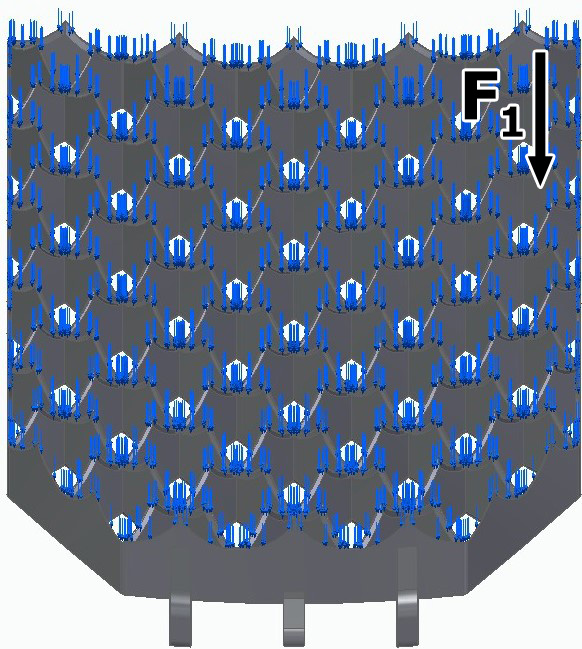
\includegraphics[width=\textwidth]{F1.jpg}
	\end{minipage}
	\hfill
	\begin{minipage}[t]{0.3\linewidth}
		\centering
		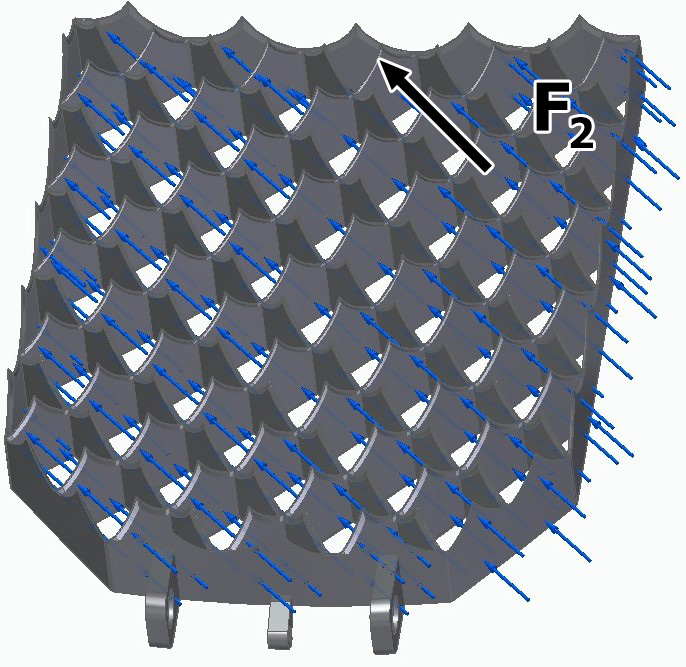
\includegraphics[width=\textwidth]{F2.jpg}
	\end{minipage}
	\hfill
	\begin{minipage}[t]{0.3\linewidth}
		\centering
		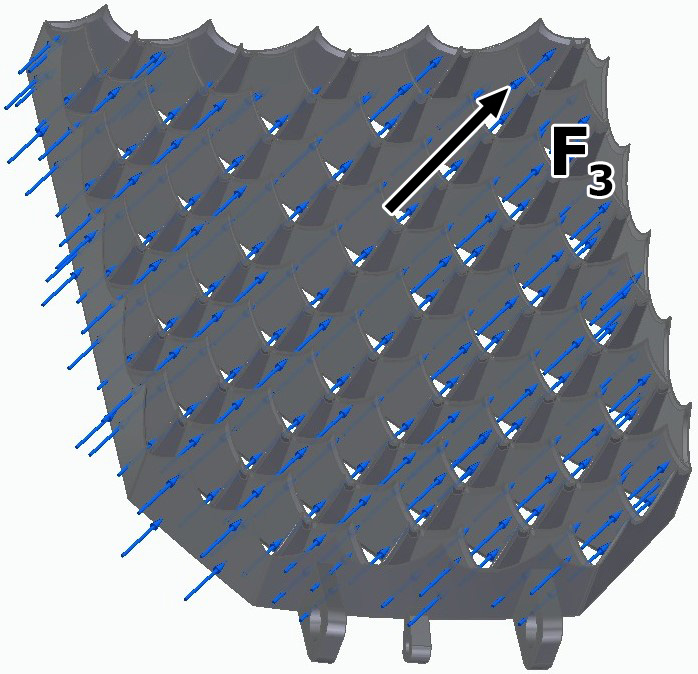
\includegraphics[width=\textwidth]{F3.jpg}
	\end{minipage}
	\caption{Aufteilung der Kräfte in die verschiedenen Richtungen}
	\label{abb_Fs}
\end{figure}\\
Der erste Anteil der Kraft ($F_1$) zeigt in Richtung der Sehne und wird auf alle Flächen der konkaven Seite gleichmäßig verteilt. Die Kräfte $F_2$ und $F_3$ liegen in der Ebene des Grid Fins, wenn die Krümmung vernachlässigt wird, und werden jeweils ebenso gleichmäßig auf die Zellwände aufgebracht, die zum Teil oder ganz senkrecht zu ihnen liegen.

Somit ergeben sich die Kräfte für die einzelnen Grid Fins wie sie in Tabelle \ref{tab_Fs} zu sehen sind
\begin{table}[ht]
	\centering
	\caption{Am Grid Fin angreifende transformierte Kräfte}
	\label{tab_Fs}
	\begin{tabular}{c||c|c|c|c}
		&D1&R1&D2&R2\\
		\hline
		$F_1/$N&$413,5$&$389,3$&$389,3$&$413,5$\\
		$F_2/$N&$6.276,0$&$4.970,8$&$-4.970,8$&$-6.276,0$\\
		$F_3/$N&$4.934,0$&$6.474,2$&$-6.474,2$&$-4.934,0$\\
	\end{tabular}
\end{table}\\~\\
Als Randbedingung werden die Innenflächen der Halterung zylindrisch festgelegt. Das heißt, dass die dort liegenden Knoten sich weder axial noch radial bewegen jedoch um die Achse drehen können.
\subsection{Optimierung der Halterung}
Bei beiden Pfeilungstypen lässt sich für alle Lastfälle sofort erkennen, dass es zu massiven Lastspitzen an der Halterung kommt. Währenddessen bleiben die Werte im Gitter deutlich niedriger, was in Abbildung \ref{abb_V1-D1} am Beispiel vom Grid Fin D1 in der Berg-Konfiguration zu sehen ist. Die hohen Spannungen an der Einspannung sind durch die nachteilige Lage in der Mitte der Wände begründet, günstiger wäre eine Positionierung an den Schnittstellen. Somit würden sich nicht mehr diese hohe Biegemomente in den Wänden ausbilden. Dieser ungünstige Kraftfluss wird durch die scharfen Kanten zusätzlich verstärkt. Um nun diese Spannungsspitzen zu vermeiden, sollte, neben einer Abrundung der Kanten, die Position der Halterungen verändert werden.
\begin{figure}[h] 
	\centering
	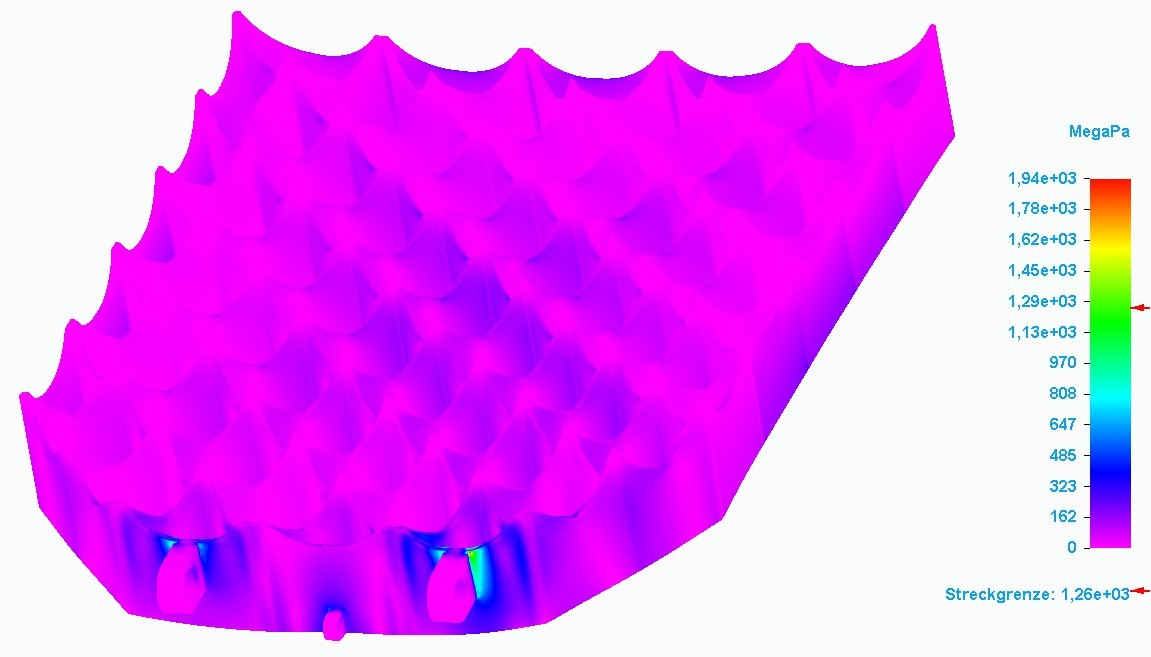
\includegraphics[width=0.9\textwidth]{D1 3.3b max 1.jpg}
	\caption{Maximale Spannungen am Grid Fin D1}
	\label{abb_V1-D1}
\end{figure}\\
Da sich die Anbringung der Halterungen genau in der Mitte einer gedachten Zelle befinden, die jedoch vom Rahmen halbiert wurde, lassen sie sich entweder tangential oder normal zum Raketenkörper verschieben, um sie auf einen Schnittpunkt der Wände zu legen. Soll Halterung B nicht in zwei Teile aufgeteilt werden, so kommt für sie nur eine Bewegung senkrecht zum Körper in Frage. Anstatt die Halterung nun in das Gitter hinein zu legen, was zu einer Verkleinerung der durchströmten Querschnittfläche führen würde und somit geringere Normalkräfte bewirken würde, werden zwei der Wände weiter fortgesetzt. Diese schneiden sich dann in der Mitte, wo die Halterung B platziert wird. Diese Halterung wird jedoch nicht direkt an der Schnittstelle konstruiert, sondern noch ein wenig weiter vom Gitter entfernt, sodass die Kraft geradliniger über die beiden Hubstangen geleitet werden kann.

Für die Halterungen A passiert das gleiche. Die nebenliegenden Gitterwände werden bis zu ihrer Schnittstelle fortgesetzt. Im Gegensatz zur Halterung B befindet sich jedoch direkt hier die Bohrung, an der der Grid Fin montiert werden soll. Somit ergibt sich der in Abbildung \ref{abb_V2-Halterung} dargestellte Aufbau.
\begin{figure}[h]
	\begin{minipage}[t]{0.45\linewidth}
		\centering
		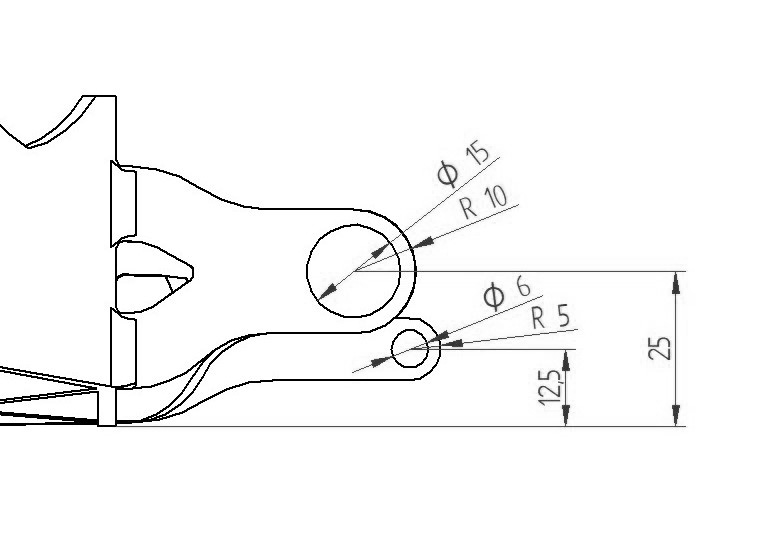
\includegraphics[width=0.85\textwidth]{Skizze Halterung 2.0 1.jpg}
	\end{minipage}
	\hfill
	\begin{minipage}[t]{0.45\linewidth}
		\centering
		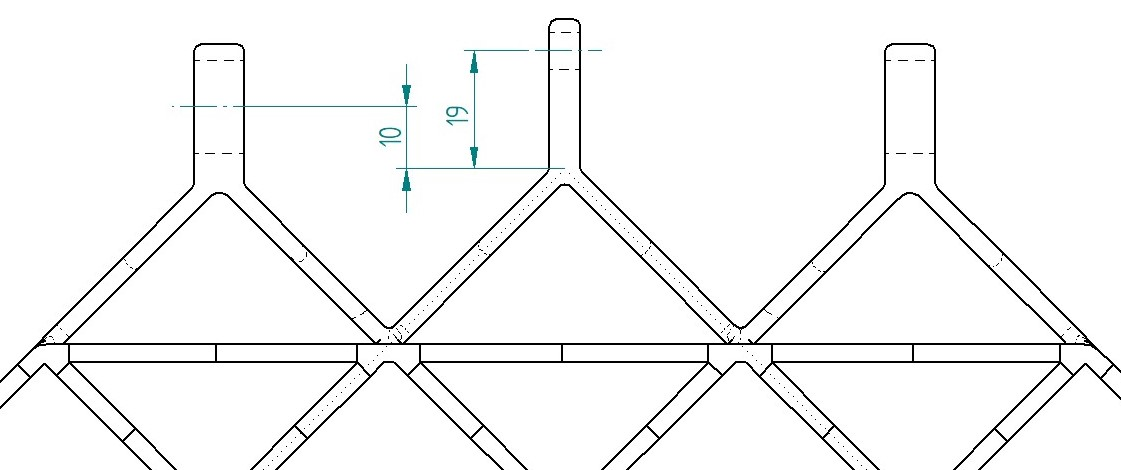
\includegraphics[width=1\textwidth]{Skizze Halterung 2.0 2.jpg}
	\end{minipage}
	\caption{Abrücken der Halterung vom Rahmen}
	\label{abb_V2-Halterung}
\end{figure}\\
Dies führt zwar schon für eine deutlichere Verbesserung, jedoch ist der Hebelarm trotz der Versetzung der Halterung B recht kurz. Dies sorgt dafür, dass direkt an der Bohrung noch immer Spannungsspitzen auftreten, die die Streckgrenze von $R_{p, 0.2} = 1.262$ MPa unterschreiten.

Um dem Hebelarm zu verlängern, wird die Halterung B auf die Höhe der konvexen Seite verlagert. Dies erzielt nun den gewünschten Effekt, dass die Spannung im Material deutlich niedriger wird. Bei allen Grid Fins treten nur noch Spannungen auf, die deutlich unter der Streckgrenze des Materials liegen und somit den Belastungen im Einsatz standhalten.
\\~\\
Somit wäre die Auslegung der Halterung nach den aerodynamischen Kräften theoretisch abgeschlossen. Jedoch muss hierbei auch noch auf die Aktuatorik und das maximale Lastvielfache geachtet werden. In der gezeigten Konfiguration hat der Grid Fin eine Masse von $m = 3,5$ kg und der Massenschwerpunkt liegt $185$ mm von der Halterung A entfernt. Mit dem Lastvielfachen von ca. 20 beim Auslösen des Ballutes entsteht nun also ein Moment von ungefähr $M=127$ Nm, welches von der Halterung B kompensiert werden muss. Die Halterung B ist an der Spindelstange montiert und leitet somit die Kraft an diese weiter. Der Hebelarm der Halterung B und die maximal ertragbare Axialkraft der Spindel müssen also aufeinander abgestimmt sein. Maxon Motoren stellt nur Spindeln mit Axiallasten von bis zu $2.700$ N her, welche folglich einen Hebelarm von $\frac{127Nm}{2700N}=47$ mm erfordert. Dies ist für den Grid Fin noch technisch machbar, weshalb ein Exemplar von diesem Anbieter gewählt wird. Der Wert liegt laut dieser Rechnung zwar minimal darüber, jedoch wird das Lastvielfache von 20 gar nicht wirklich erreicht, sodass die Rundung annehmbar ist. Da die Hubstange gelenkig mit dem Grid Fin verbunden ist, ist zu beachten, dass nur der Abstand der Halterungen in Sehnenlänge als effektiver Hebelarm wirkt. Somit werden sie im Gegensatz zum Aufbau aus Abbildung \ref{abb_V2-Halterung} gleich weit vom Rahmen entfernt platziert. Wird die Verbindungsstange zwischen Halterung und Hubstange auf die gleiche Länge wie der Hebelarm gesetzt, ist der Hub für den gegeben Abstand der Halterungen minimal. Um auf den gewünschten Hebelarm zu kommen, werden beide Halterungen noch ein wenig an die Hinter- und Vorderkante des Grid Fins gelegt, sodass sich die endgültige Geometrie, wie sie in Abbildung \ref{abb_Halterung-fertig} zu sehen ist, ergibt. Zusätzlich befinden sich noch Kanten und Nuten in den Bohrungen zur Befestigung der Lagerung, auf welche im weiteren Verlauf dieser Arbeit in Detail eingegangen wird.
\begin{figure}[h] 
	\centering
	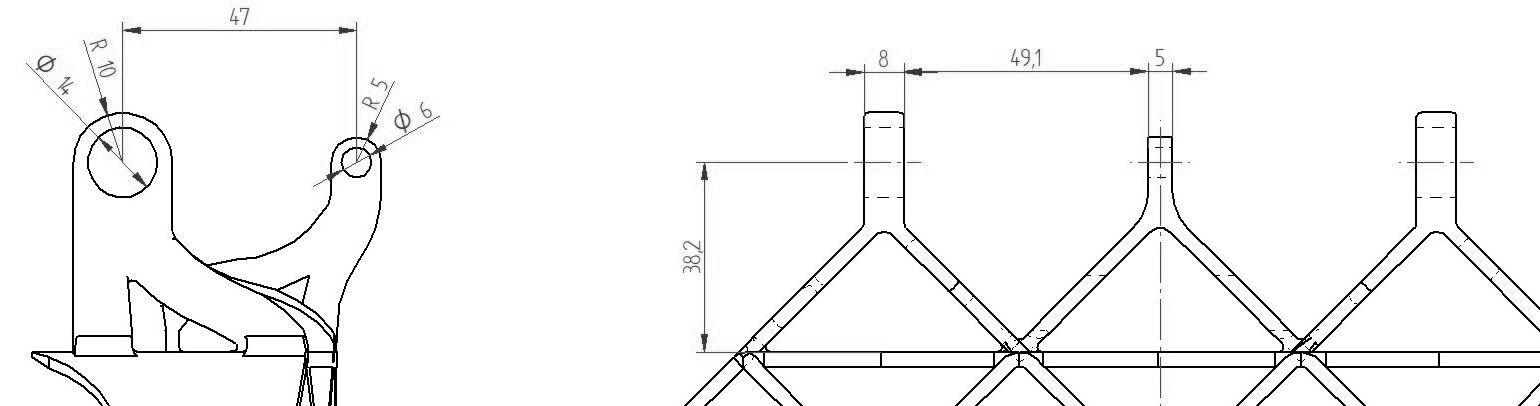
\includegraphics[width=0.9\textwidth]{Skizze Halterung 3.6.jpg}
	\caption{Endgültige Geometrie der Halterung}
	\label{abb_Halterung-fertig}
\end{figure}\\
Zur Bestätigung werden wieder FEM-Analysen durchgeführt und diesmal werden ergänzend zu den aerodynamischen Kräften auch in einem separaten Lastfall die Beschleunigungskräfte untersucht, die auf dem gesamten Volumen in Richtung der Pfeilungsspitzen wirkt. Bei den Lastvielfachen werden die anderen Kräfte vernachlässigt, da sie auf Grund ihrer Wirkung in Gegenrichtung eine Stützwirkung haben und somit die Spannungen nur weiter senken würden. Beim Auftreten der ruckartigen Abbremsung durch den Ballonschirm ist der Max Q bereits überschritten und somit sind die anderen Kräfte nur noch deutlich geringer. Wie Abbildungen \ref{abb_Halterung_max} und \ref{abb_Halterung_20g} zeigen, wird die Streckgrenze weiterhin nicht überschritten. Somit gilt die Halterung als bestätigt.
\begin{figure}[h]
	\begin{minipage}[t]{0.5\linewidth}
		\centering
		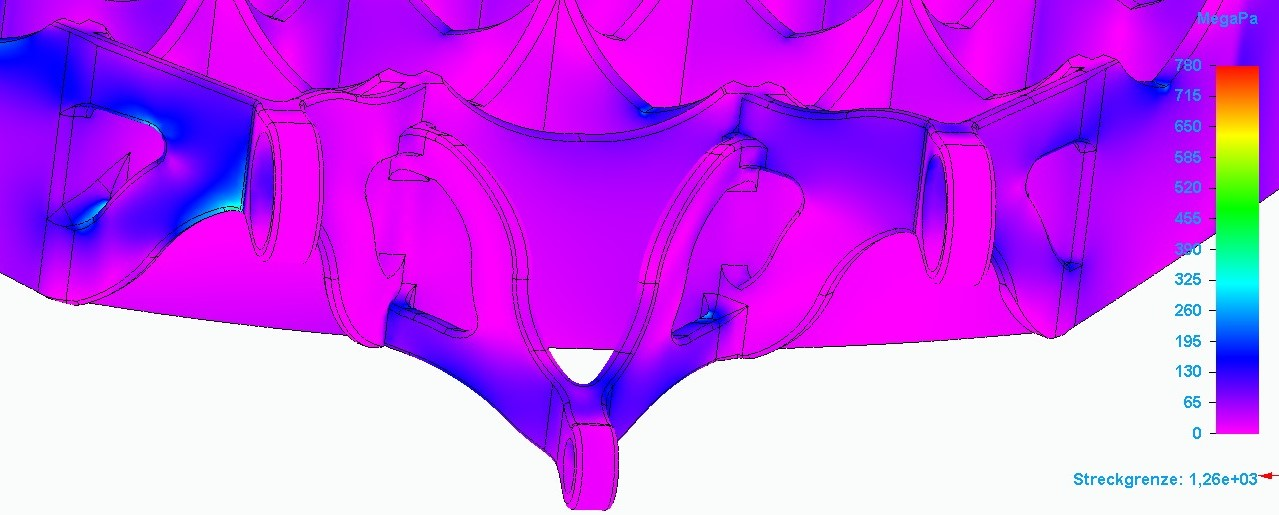
\includegraphics[width=0.95\textwidth]{D2 3.6.2 b Halterung.jpg}
		\caption{Maximale Belastungen an der endgültigen Geometrie der Halterung}
		\label{abb_Halterung_max}
	\end{minipage}
	\hfill
	\begin{minipage}[t]{0.41\linewidth}
		\centering
		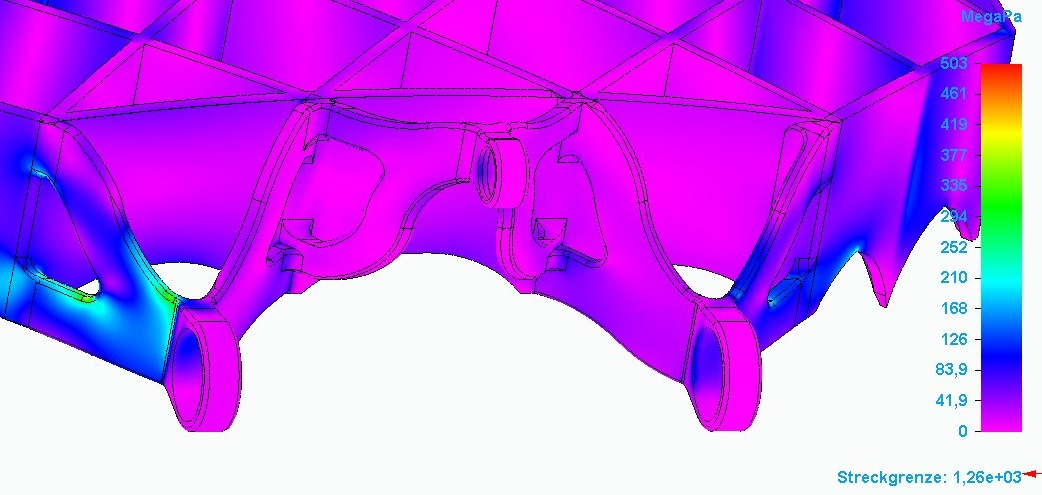
\includegraphics[width=\textwidth]{20g 3.6.2 b.jpg}
		\caption{Belastungen an der endgültigen Geometrie der Halterung beim maximalen Lastvielfachen}
		\label{abb_Halterung_20g}
	\end{minipage}
\end{figure}
\subsection{Optimierung des Gitters}
Als nächstes wird das Gitter untersucht. Es ist sofort erkennbar, dass die Belastungen über das Gitter verteilt relativ niedrig und deutlich unter der Streckgrenze liegen. Unabhängig vom Tal- oder Berg-Tyous sind die auftretenden Spannungsspitzen keinesfalls kritisch. Somit ist eine Aufdickung des Materials nicht nötig, sondern es kann über eine Reduzierung der Wandstärke nachgedacht werden.

Die Maximale Reduktion der Wanddicke hängt wohl von den mechanischen als auch thermischen Belastungen ab. Letzteres ist jedoch ein sehr komplexes Phänomen, das von der Zusammensetzung der Atmosphäre, den zeitlich sich ändernden Strömungsbedingungen, der Position des Verdichtungsstoßes und dem Aufbau des Grid Fins abhängt, sodass dieser Aspekt nicht auch nur überschlägig in dieser Arbeit behandelt wird. Dies gilt es somit in nachfolgenden Arbeiten zu überprüfen.
\\~\\
Der Grid Fin ist momentan am von der Rakete weg zeigenden Ende nur $1,5$ mm dick, was für den Wiedereintritt schon ein gefährlich kleiner Wert sein könnte. Deswegen soll dieser zunächst nicht unterschritten werden. Es ist jedoch auch kein signifikanter Anstieg der Spannungen zur Halterung hin zu erkennen, der den Verlauf der Wanddicke rechtfertigt. Deswegen werden zunächst alle Wände im Gitter auf eine Dicke von $d_G = 1,5$ mm gesetzt, während die Wandstärke und die Wände, die außerhalb des Gitters zu den Halterungen führen, unverändert bleiben. Dies scheint nach einer ersten FEM-Analyse die Belastung des Materials nicht stark zu verändern, sodass auch Rahmen- und Halterungswände auf diesen Wert hinabgesetzt werden. Die Spannungen in den Grid Fins liegen für alle Positionen und auch beim maximalen Lastvielfachen weit unter der Streckgrenze von $R_{p, 0.2} = 1262$ MPa. Die höchsten Spannungen treten beim Grid Fin des Tal-Typus in der Position D2 auf. Dieser ist in Abbildung \ref{abb_V100} dargestellt und zeigt, dass die maximale Spannung gerade so noch unter $800$ MPa liegt.
\begin{figure}[h] 
	\centering
	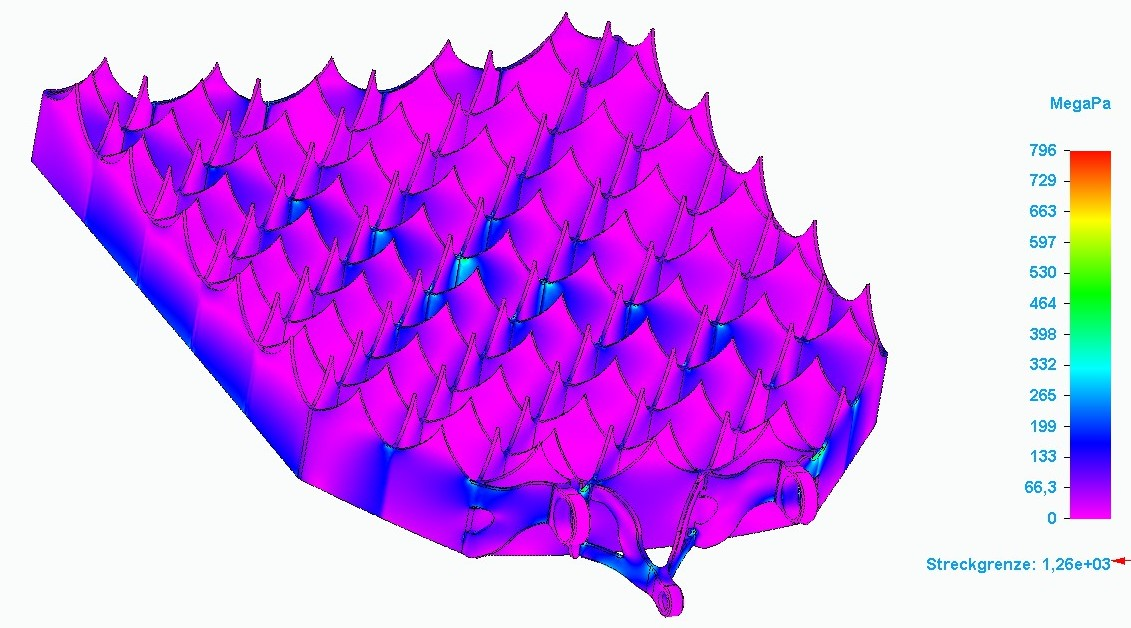
\includegraphics[width=0.8\textwidth]{D2 3.9 t.jpg}
	\caption{Spannungen am Grid Fin D2 mit konstante Wanddicke von $1,5$ mm beim maximalen Lastfall}
	\label{abb_V100}
\end{figure}\\
Somit resultiert ein Sicherheitsfaktor von über 1,5. So hohe Spannungen treten jedoch nur an einzelnen Stellen auf, die hauptsächlich am Berührungspunkt der Halterung mit dem Rahmen oder direkt an der Halterung liegen. Im Gitter sind für alle Belastungsfälle die Spannungen geringer und bleiben großteils unter 200 MPa. Deutlich sind außerdem zwei diagonale Streifen, die sich in der Mitte des Gitters treffen, zu erkennen, in denen ebenso wie am Rahmen etwas höhere Belastungen auftreten. Aber selbst das Maximum in der Mitte ist mit Spannungen knapp über 300 MPa noch immer ungefährlich.
\\~\\
Der Vergleich von der Berg- und Tal-Konfiguration zeigt, dass keine signifikanten Unterschiede auftreten. Die maximalen Spannungen sind beim Tal-Typus zwar immer etwas größer, aber nur um insignifikante kleine Beträge, dass es keine Rolle spielt. Deswegen muss an der Stelle wieder thermisch argumentiert werden. Beim Tal-Typus sind die Spitzen isolierte der Strömung entgegenzeigende Punkte. Beim Berg-Typus hingegen liegen die Spitzen der sich kreuzenden Wände aufeinander, sodass die Wärme an ein größeres Volumen abgegeben werden kann. Unter der Annahme, dass der Berg-Typus somit thermisch robuster ist, wird dieser hier als die endgültige Geometrie des Grid Fins ausgewählt. Ein Rendering dieser finalen Geometrie ist in Abbildung \ref{abb_rendering1} gezeigt.
An dieser Stelle sei noch zusätzlich zu erwähnen, dass folglich auch die Ideen zur Integrierung von Hohlräumen verworfen werden müssen. Unabhängig vom Zweck zur Kühlung, Druckmessung oder einfach nur Gewichtseinsparung erlaubt die geringe Wanddicke keinen Platz für solche Strukturen. Momentan wird der Selektive-Laserschmelz-Prozess des Anbieters Rapid Object GmbH betrachtet, der einer minimale Wandstärke von einem Millimeter bedarf. Somit kann nur bei Wandstärken $d>2$ mm über Hohlräume nachgedacht werden. Es gibt zwar auch Anbieter, die eine bessere Auflösung ermöglichen, jedoch würde dies die ohnehin schon hohen Produktionskosten weiter steigern. Die spitzen Kanten der Zellwände liegen zwar auch unter der Mindestwanddicke, aber sie können je nach Lage des Grid Fins im Drucker noch immer teilweise dargestellt werden. Es wird vermutlich nur zu einer stärkeren Abrundung der Vorder- und Rückkante kommen, sodass der Widerstand minimal ansteigt, aber keine weiteren Nachteile entstehen. Trotz des Ausschließens von Hohlräumen beläuft sich die finale Masse der Grid Fins mit der Reduzierung der Wandstärke auf $2,8$ kg. Damit sind auch die Trägheitskräfte reduziert, was eine geringere Belastung der Ausklappaktuatorik bewirkt. Eine Möglichkeit wäre es, eine schwächere Spindel zu nehmen, jedoch ist es vorteilhafter, stattdessen den Hebel der Halterung B auf eine Länge von $37,5$ mm anzupassen. Dadurch bleiben die Spannungen in der Spindelstange zwar in derselben Größenordnung wie zuvor, aber der benötigte Hub verkürzt sich. Dies bewirkt Material- und Masseeinsparungen für einen Großteil der Bauteile. So kann zum Beispiel das vordere Kegellager verkleinert werden, da die Hubstange näher an die Wellenachse rückt. Da die Geometrie des Grid Fins wieder geändert wurde, werden nun erneut FEM-Simulationen durchgeführt, die jedoch keine signifikante Verschlechterung zeigen.
Eine ergänzende vollständige Sammlung der Ergebnisse der FEM-Analysen aller Belastungszustände am Grid Fin befindet sich im Anhang \ref{sec:mehrFEM}.
\begin{figure}[h] 
	\centering
	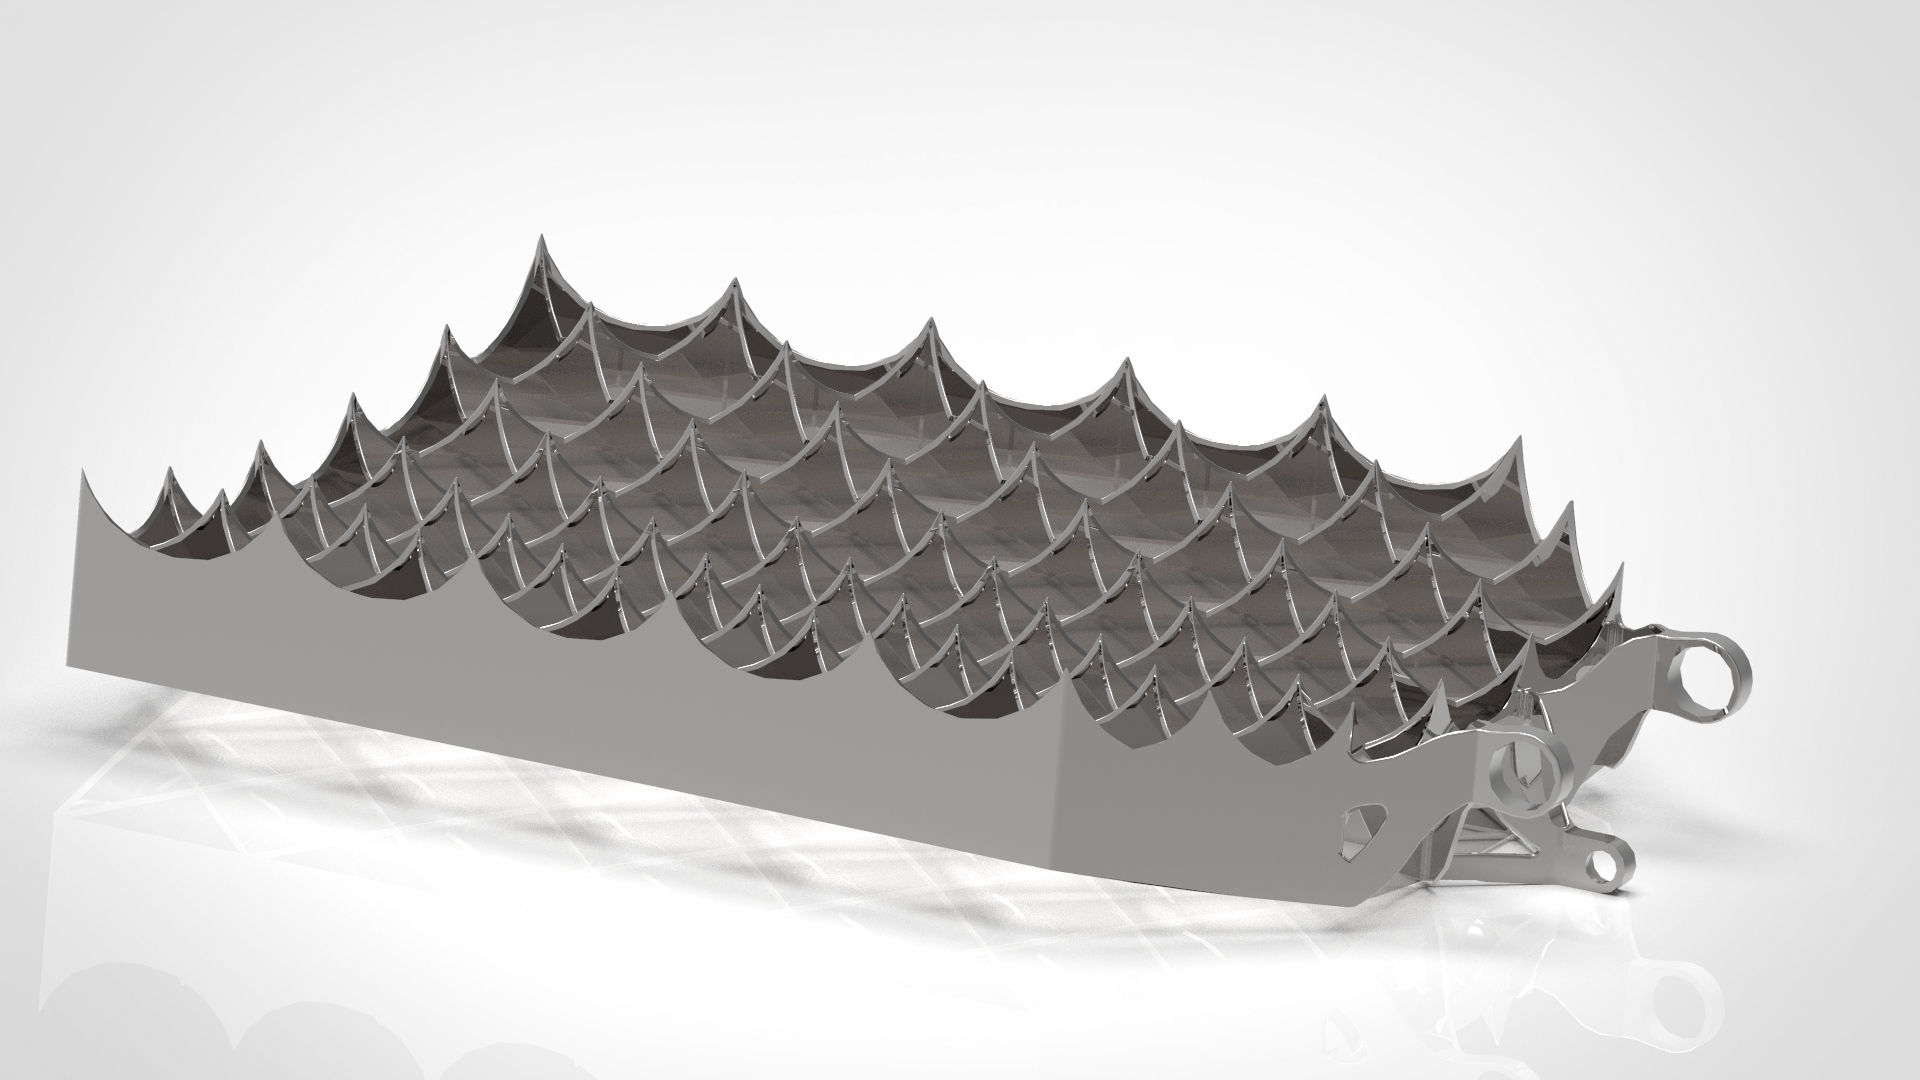
\includegraphics[width=0.8\textwidth]{Grid_Fin_Render.3.jpg}
	\caption{Finaler Grid Fin aus Edelstahl}
	\label{abb_rendering1}
\end{figure}\\
Da eine Gewichtsreduzierung der Grid Fins weitreichende Folgen für die Gesamtmasse des Systems hat, kann noch mal über die Werkstoffwahl nachgedacht werden. Titan wurde trotz seiner deutlich geringeren Dichte als Edelstahl ausgeschlossen, weil er signifikant teurer ist. Sollte sich jedoch herausstellen, dass die Einsparungen der Masse die Kosten überwiegen, sollte diese Entscheidung überdacht werden.

Ein Titan Grid Fin besäße nur eine Masse von $m=1,6$ kg, wodurch sich sein Hebelarm auf $21,5$ mm verkürzen lässt. Die restliche Geometrie des Grid Fins bleibt unverändert und die FEM-Berechnungen ergeben, dass maximale Spannungen von $889$ MPa beim Grid Fin D2 auftreten, also leicht über den Belastungen des Edelstahl Grid Fins, aber nicht bedeutend.

Durch ein Verkürzen des Hebelarms kann nicht nur die Spindelstange kürzer werden, sondern auch ihre Achse muss nach unten gelegt werden. Dies führt jedoch zu Komplikationen, da nun das Linearlager in der Achse der Welle liegt. Dadurch kommt es zu einer sehr ungünstigen Wellenform, die nur einen schlechten Kraftfluss erlaubt und zu hohen Biegemomenten führt. Des Weiteren muss dadurch das Gehäuse größer dimensioniert werden. Somit geht wiederum mehr Bauraum innerhalb der Rakete verloren. Ein weiteres Problem stellt die Vorderseite der Welle dar. Theoretisch erlaubt die niedrigere Hubstange ein kleineres Kegellager zu verwenden, jedoch rückt durch den kürzeren Hub das Linearlager nach vorne, was den Bauraum blockiert. Ein kleineres Lager würde nicht mal die Masse der Welle reduzieren, da die Außenschicht nur nach innen auf die Position des Hohlraums rückt. Selbst der Effekt des geringeren Umfangs wird dadurch negiert, dass der Bereich hinter der Auflagefläche des Lagers nicht mehr gut erreichbar ist und sich deswegen dort weniger aushöhlen lässt. Wegen der Biegespannung in der Verbindungswelle kann die Breite im vordersten Teil der Welle auch nicht reduziert werden. Ein Abtragen des Materials auf der Oberseite führt hingegen zu einer flacheren Fläche, die beim Start in die Strömung zeigt und somit unnötig viel Widerstand verursacht. Wegen all dieser Gründe würde sich eine weitere Reduzierung des Helbelarms von Halterung B nicht rentieren. Sollte jedoch ein Titan Grid Fin mit der gleichen Halterungsgeometrie verwendet werden, ergäbe sich noch immer der Vorteil der um ca. 1,2 kg verringerten Masse. Dies wiegt jedoch nicht die hohen Kosten des Materials auf, weswegen weiterhin Edelstahl als Werkstoff verwendet wird. Der Grid Fin aus Stahl würde im 3D-Druck knapp 13.000€ Kosten, während der Preis bei Titan im Bereich von mehren 10.000€ liegt und somit ungefähr das dreifache kostet.
\section{Bestätigung der mechanischen Belastbarkeit der Aktuatorik}
Mit der Festlegung des Grid Fin Aufbaus, insbesondere der Halterung, kann überprüft werden, ob auch alles auf der Wellenseite den mechanischen Lasten standhält. Hierfür werden die Kräfte, die an den einzelnen Halterungen wirken, benötigt.
\begin{figure}[h] 
	\centering
	\includegraphics[width=0.5\textwidth]{Halterungkräfte1.png}
	\caption{Kräfte an den Halterungen}
	\label{abb_richtungen_Halterungskräfte}
\end{figure}\\
Wie in Abbildung \ref{abb_richtungen_Halterungskräfte} zeigt werden für die Kräfte der Halterungen drei neue Richtungen definiert.Die erste ist die $\xi$-Richtung, die identisch mit der für die FEM-Berechnung definierten Kraftrichtung $F_1$ ist. $\eta$ zeigt von der Mittelachse der Rakete zum betrachteten Grid Fin. Folglich ergibt sich als letztes die $\zeta$-Richtung tangential zum Raketenrumpf und vervollständigt das Rechtssystem. Zusätzlich muss nun zwischen den beiden Halterungen A unterschieden werden. A2 liegt in positiver $\zeta$-Richtung von A1.

 Wenn angenommen wird, dass die Halterung B, da sie deutlich weniger steif als die Halterungen A ist, nur Belastung in $\eta$-Richtung aufnehmen kann, ergeben sich die Kräfte wie in Tabelle \ref{tab_Haltekräfte} dargestellt. Links sind Kräfte am Grid Fin R1 dargestellt, was die höchste Belastung für das Lager A bedeutet, und rechts R2 mit der höchsten Belastung für Lager B. Die detaillierte Rechnung befindet sich im Anhang \ref{sec:halterkraefte}. 
\begin{table}[h] 
	\centering 
	\caption{Kräfte an den Halterungen der Grid Fins}
	\label{tab_Haltekräfte}
	\begin{tabular}{c|r|r|rc||c|r|r|r} 
		\textbf{R1}&$F_{\zeta}$/N&$F_\eta$/N&$F_\xi$/N&&\textbf{R2}&$F_{\zeta}$/N&$F_\eta$/N&$F_\xi$/N\\ 
		\hline 
		A1& 612,00&-6.319,94&-531,55&&A1&599,90&233,47&-474,45\\
		A2&-1.001,31&-2.342,88&-531,54&&A2&-1.013,41&3.783,28&-474,45\\
		B&0&-401,16&0&&B&0&3.783,28&0\\
	\end{tabular}
\end{table} \\
Für die Bauteile, die nicht so hohen Lasten wie der Grid Fin ausgesetzt sind, wird im Folgenden nicht mit den Werkstoffwerten des teuren Edelstahls 1.4542 gerechnet. Für die Teile, die nicht mit der Strömung in Kontakt kommen, wird stattdessen die Aluminiumlegierung 3.3321 mit $R_{p,0.2} = 280$ MPa verwendet, und für die anderen Bauteile, wie weiterhin auch hohen thermischen Lasten ausgesetzt sind, wird der Edelstahl 1.4401 mit einer Streckgrenze von $R_{p,0.2} = 400$ MPa angenommen. Dies ist ein Kompromiss aus Festigkeit und Materialkosten. Noch günstigere Werkstoffe hätte eine geringere Festigkeit, weswegen wieder mehr Material benötigt werden würde. Dadurch steigt die Masse und als weitere Folge auch der Preis.
\subsection{Lager der Halterung}
Für die Lasten an den Lagern ist nur die Aufteilung in Radial- $F_r$ und Axialkraft $F_a$, wie sie in Tabelle \ref{tab_lagerkraefte} zu sehen ist, von Bedeutung. Dabei sei noch zu bedenken, dass die Kraft in $\xi$-Richtung auf Grund des Aufbaus nur von einem der A Lager kompensiert werden kann. Auch wenn dieser Umstand für die vorherige Berechnung keine Rolle spielte, da die beiden Halterungen A auf einer Achse liegen, wird es im Folgenden berücksichtigt.
\begin{table}[h] 
	\centering 
	\caption{Lagerkräfte in den Halterungen}
	\label{tab_lagerkraefte}
	\begin{tabular}{c|r|rc||c|r|r} 
		\textbf{R1}&$F_{r}$/N&$F_a$/N&&\textbf{R2}&$F_{a}$/N&$F_r$/N\\ 
		\hline 
		A1& 6.349,50&-1.063,10&&A1&643,73&-948,90\\
		A2&2.547,89&0&&A2&3.916,65&0\\
		B&401,16&0&&B&4.861,12&0\\
	\end{tabular}
\end{table} \\
Aus diesen Werten lässt sich nun über die Flächenpressung und Abscherung der erforderliche Durchmesser $D$ und die benötigte Auflagebreite $B$ der Hilfswelle bestimmen. Für die Abscherung gilt
\begin{equation}
	\tau_{\mathrm{zul.}}\leq\tau_\mathrm{scher}=\frac{F_r}{m\pi D^2/4}.
\end{equation}
Mit $\tau_{\mathrm{zul.}}=R_{p, 0.2}\cdot 0,6$ \cite{metall} und $m$ als die Anzahl der Schnittflächen lässt sich der Mindestdurchmesser bestimmen.
\begin{equation}
	D \leq \sqrt{\frac{4F}{m\pi 0,6 R_{p, 0.2}}}
\end{equation}
Für die Halterung A ist $m_A =1$, sodass eine Mindestdicke von $D_A =5,8$ mm benötigt wird, woraus sich der sich eine Auflagebreite von $B_A = 3,3$ mm ergibt. Da sich der Aufbau des Grid Fins seit dem ersten Modell verändert hat, muss auch die Anbringung an der Welle, welche in Abbildung \ref{abb_Welle} zu sehen war, angepasst werden. Durch die Verlegung der Halterung A rückt der Grid Fin näher an den Raketenkörper. Statt nun Greifarme aus der Welle herausragen zu lassen, wird diese nur ein wenig verlängert, sodass die Verbindungslinie durch die beiden Halterungen A die Welle durchstößt. Auf diese Verbindungslinie wird eine Stange, im Weiteren Verbindungswelle genannt, mit einem Durchmesser von $D_\mathrm{Verbindungswelle} = 10$ mm gelegt, auf der der Grid Fin montiert wird. Diese Variante der Halterung hat zum einen den Vorteil, dass keine komplizierte Greiferstruktur gefertigt werden muss, und zum anderen steht ein Großteil der planaren Rahmenwand im eingeklappten Zustand nicht mehr direkt in der Strömung, sondern im Windschatten der Welle. Dadurch wird ungewollter Widerstand und Belastung der Grid Fins verhindert. Um den Grid Fin reibungsarm zu sichern, muss er sowohl axial als auch radial mit Wälzlagern gelagert werden. Zylinderrollenlager, wie sie schon bei der Welle verwendet werden, sind hier jedoch eine ungünstige Wahl, da sie einen recht großen Bauraum benötigen. Stattdessen zeigt Abbildung \ref{abb_Lager_HA} wie die Halterung A auf beiden Seiten mit einem schmalen Nadellager radial  und mit einem Kugellager axial mit der Welle verbunden ist. Diese Kombinationslager werden von außen mit Nutmuttern, die auf die Verbindungswelle aufgeschraubt und durch Sicherungsbleche gesichert sind, an den Grid Fin gedrückt. Um ein Verrutschen der Verbindungswelle in der Welle zu verhindern, muss diese noch durch eine Passschraube fixiert werden. Für diese Passschraube werden wieder aus der Flächenpressung und der Abscherung die Mindestmaße des Durchmessers und der Breite bestimmt. Mit einem Durchmesser von $D_\mathrm{Passschraube} = 10\mathrm{ mm}> 1,2$ mm und einer Kontaktbreite von $B_\mathrm{Passschraube} = 8\mathrm{ mm}> 1,3$ mm ist sie für diese Anwendung ausreichend.
\begin{figure}[h] 
	\centering
	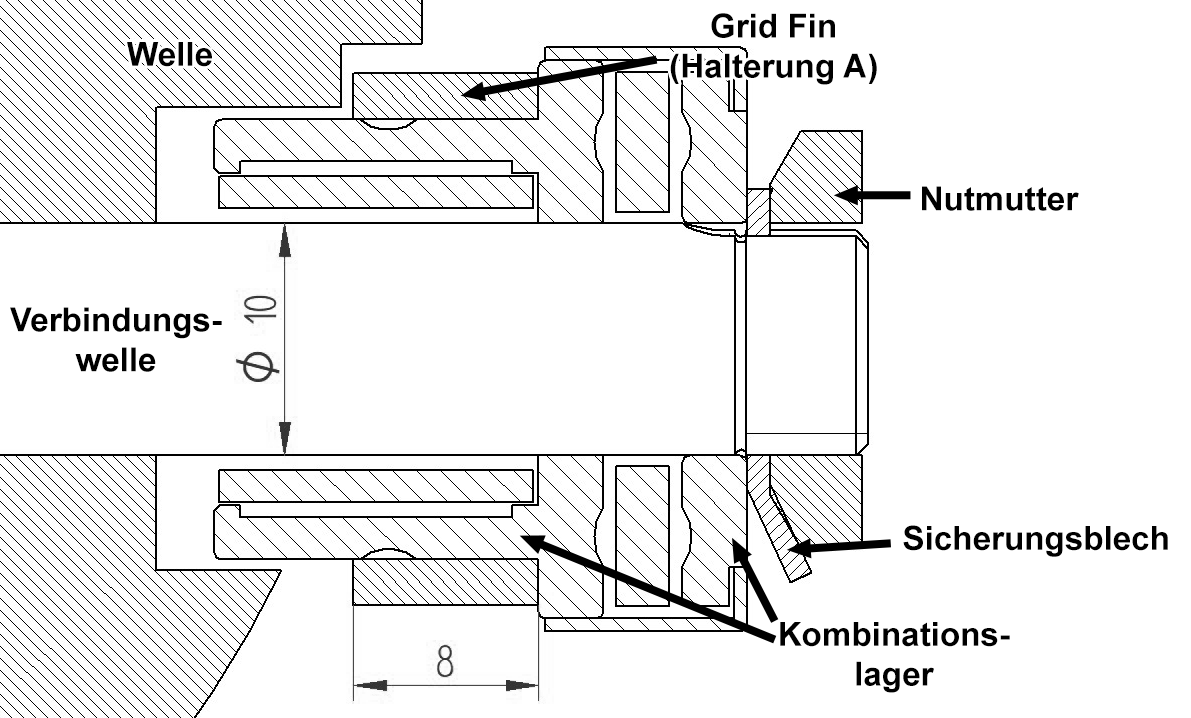
\includegraphics[width=0.75\textwidth]{Skizze Halterung A.png}
	\caption{Lagerung der Halterung A}
	\label{abb_Lager_HA}
\end{figure}\\
Die Halterung B wird von beiden Seiten gestützt, sodass mit $m_B = 2$ mm ein Mindestdurchmesser von $D_B = 3,6$ mm errechnet wird. Die zugehörige Breite beläuft sich somit auf $B_B = 4,1$ mm. Wie schon angemerkt, treten hier kaum Axialkräfte auf, sodass ein Rillenkugellager ausreicht, um diese aufzunehmen. Es wird auf der einen Seite gegen eine Schulter in der Halterung B des Grid Fins gedrückt und auf der anderen Seite durch einen Sicherungsring fixiert. Zwei Stifte werden von beiden Seiten gegen die innere Kante des Lagers gedrückt und miteinander verschraubt. Diese Stifte können anschließend von außen mit Muttern an die Verbindungsstange für den Hub fixiert werden, sodass sich der Aufbau wie in Abbildung \ref{abb_Lager_HB} ergibt. Es werden normale Muttern verwendet, da sie keiner Last ausgesetzt sind, die eine Verdrehung bewirken könnte. Somit ist auch die Halterung B axial und radial bestimmt, kann sich aber noch immer reibungsarm um ihre Achse drehen. Das Kugellager hat zwar nur eine Breite von 3mm, was unter dem Wert liegt, der sich aus der Flächenpressung ergeben hat. Jedoch wurde dort mit dem Mindestdurchmesser gerechnet, sodass, wenn passend zum Innendurchmesser des Kugellagers die Rechnung mit $D_B = 5$ mm wiederholt wird, nur noch eine Breite von $B_B =2,9$ mm benötigt wird. Diese Lagerung wird genauso auch ein zweites Mal auf der anderen Seite der Verbindungsstange verwendet.
\begin{figure}[h] 
	\centering
	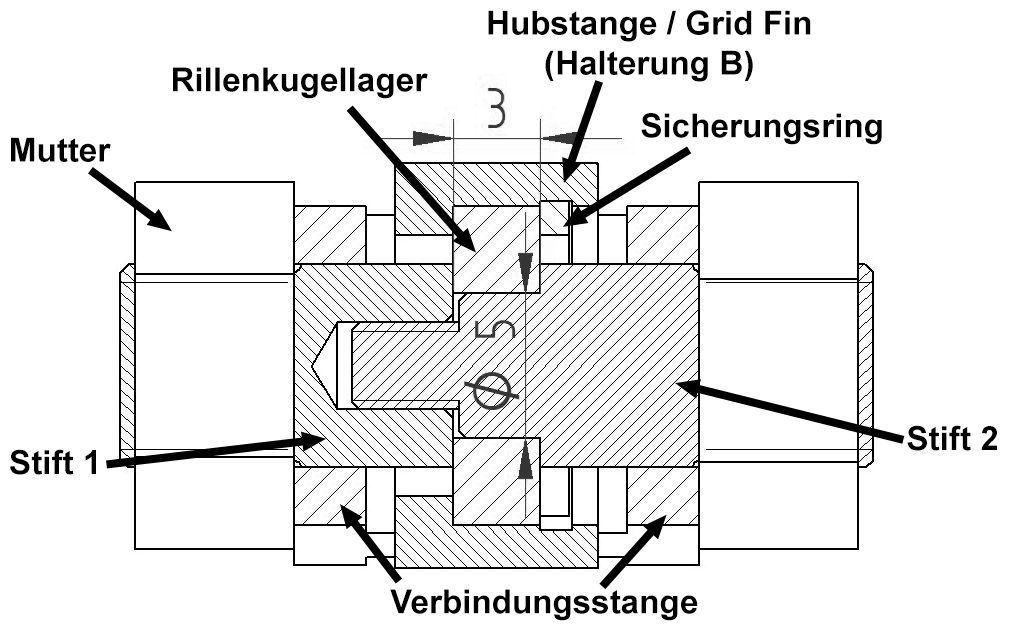
\includegraphics[width=0.75\textwidth]{Skizze Halterung B.png}
	\caption{Lagerung in der Halterung B}
	\label{abb_Lager_HB}
\end{figure}
\subsection{Lagerung der Welle}\label{sec:lagerWelle}
Als nächstes wird die Lebensdauer der Lagerung der Welle überprüft, da diese sich auch unter Last bewegen müssen. Hierzu werden zunächst über das Kräftegleichgewicht die Lasten in den beiden Kegelrollenlagern bestimmt.
\begin{figure}[h] 
	\centering
	\includegraphics[width=0.9\textwidth]{Skizze Lager.png}
	\caption{Lagerkräfte an den Kegelrollenlagern}
\end{figure}\\
Für den Fall, dass die am Grid Fin angreifende Axialkraft in positive $\eta$-Richtung zeigt, ist die Axialkraft am vorderen Kegellager $F_{a, \mathrm{K1}} = 0$ und am hinteren $F_{a, \mathrm{K2}} = F_\eta$. Da es für den anderen Fall genau umgekehrt ist, wird bei der Untersuchung der maximalen Belastung für beide Lager angenommen, dass sie jeweils die Axiallast aufnehmen. Die Radialkräfte ergibt sich aus der Kraft in $\zeta$- und $\xi$-Richtung und lässt sich mit dem Kräfte- und Momentengleichgewicht bestimmen.
\begin{equation}\label{eq_lagerWelle1}
	F_{r, \mathrm{K1}} = F_r\cdot\frac{208\mathrm{mm}}{265\mathrm{mm}}=6.359,5\mathrm{N}
\end{equation}
\begin{equation}\label{eq_lagerWelle2}
	F_{r, \mathrm{K2}} = F_r-F_{r, \mathrm{K1}}=1.742,7\mathrm{N}
\end{equation}
Aus den Lasten in den Lagern und den in den Herstellerangaben genannten statischen Tragzahlen lässt sich die äquivalente Belastung berechnen. Mittels der ebenfalls vom Hersteller gegebenen dynamische Tragzahl ergibt sich dann für das vordere Kegellager eine Lebensdauer von über 1.000 Stunden und für das hinter sogar das Fünffache \cite{metall}. Es wurde dabei mit der maximal auftretenden Drehzahl, die sich aus der in Kapitel \ref{sec:betriebssim} beschriebenen Betriebssimulation ergibt, gerechnet. Trotzdem liegt der Wert noch immer deutlich über der benötigten Lebensdauer. Dies liegt jedoch daran, dass die Größe der Lager sich aus der Geometrie der Welle und des Grid Fins anstatt aus den Belastungen ergeben hat, wodurch kein kleines Modell in Frage kommt. Bei den gewählten Exemplaren wurde schon versucht die preislich günstigste Option zu wählen, sodass ihre Größe nicht zu sehr zum Nachteil wird.
\subsection{Belastung der Welle}
Die Welle selbst hat zum einen den groben Aufbau, wie er in Abbildung \ref{abb_Welle} zu sehen war, zum anderen zeigt Abbildung \ref{abb_aufbau_Welle} wie sie an einigen Stellen von dieser rotationssymmetrischen Geometrie abweicht.
\begin{figure}[h] 
	\centering
	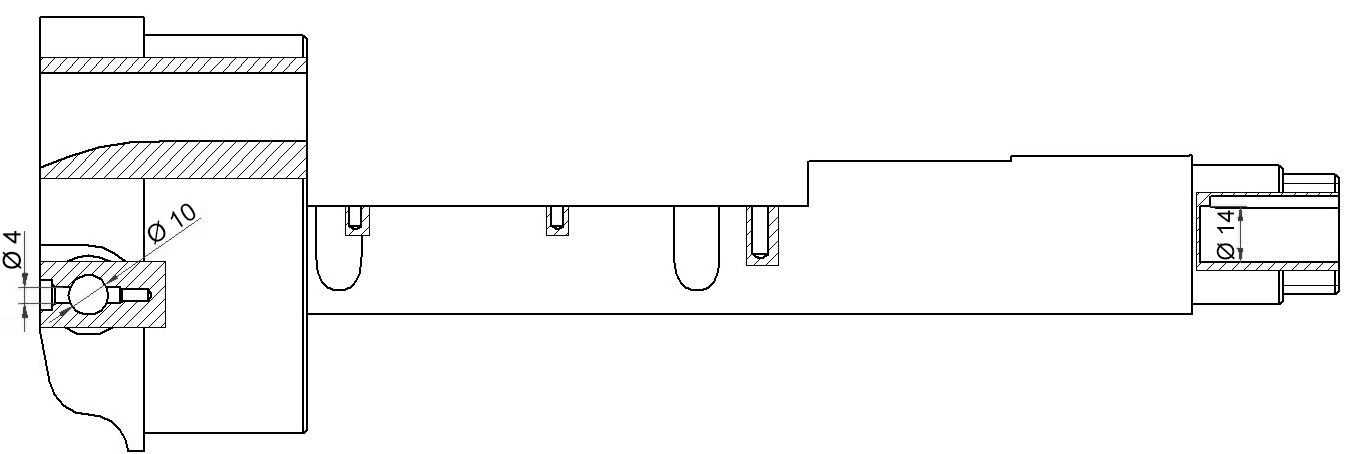
\includegraphics[width=0.9\textwidth]{Skizze Welle ausbruch.jpg}
	\caption{Aufbau der Welle}
	\label{abb_aufbau_Welle}
\end{figure}\\
 Ein Aspekt ist die schon im Abschnitt zu der Halterung angesprochenen Verbindungswelle, die die Welle durchstößt. Auf der gleichen Höhe, aber auf der Stirnseite befindet sich mittig eine Bohrung und Senkung für die Passfeder. Für die Hubstange existiert des Weiteren ein großer Ausschnitt durch den größten Durchmesser der Welle. Damit im eingeklappten Zustand die Berge des Grid Fins nicht gegen die Welle stoßen, ist die untere Vorderkante ausgehöhlt. Das Linearlager der Hubstange muss von unten festgeschraubt werden, sodass zunächst ein flacher Ausschnitt in die Welle eingebracht worden ist, auf der eine Platte festgeschraubt werden kann. Diese Platte wird anschließend von unten mit dem Lager verschraubt. Um ein Montieren der Schrauben zu ermöglichen, werden jedoch noch Einbuchtungen an der Welle benötigt. Am hinteren Ende der Platte befindet sich ein angewinkelter Teil, an dem das Spindelgetriebe festschraubt wird.
Für dieses und sein integrierten Motor sind auch noch Einbuchtungen in der Welle nötig. Am hinteren Ende befindet sich dann schließlich das Gewinde für die Nutmutter und die Nut für das Sicherungsblech. Schlussendlich ist an der hinteren Stirnseite der Welle eine Bohrung mit Passfedernut angebracht, in der die Welle des Getriebes montiert wird.
Für die Analyse der Welle wurden wieder FEM-Berechnungen durchgeführt. Auf den Flächen, auf denen die Lager aufliegen, werden wie schon beim Grid Fin zylindrische Bedingungen festgelegt, wobei die axiale Beschränkung nur bei jeweils einem der beiden Lager angewandt wird. Zusätzlich wird eine Drehung der Welle um ihre Achse durch ein Festhalten in tangentialer Richtung der Passfedernut am hinteren Ende verhindert.
Für die FEM-Berechnung, deren Ergebnis in \ref{abb_Well_FEM} dargestellt ist, werden die Kräfte der Halterung A an den Stellen eingeleitet, an denen die Verbindungswelle in die Welle führt, mit Ausnahme der $\xi$-Kraft, die durch die Passschraube übertragen wird. 
Die Kraft der Halterung B hingegen wird erst über das Spindelgetriebe auf die Welle übertragen. Somit greift die resultierende Kraft in der Simulation in den Bohrlöchern an, an denen die Spindel befestigt ist.
\begin{figure}[h] 
	\centering
	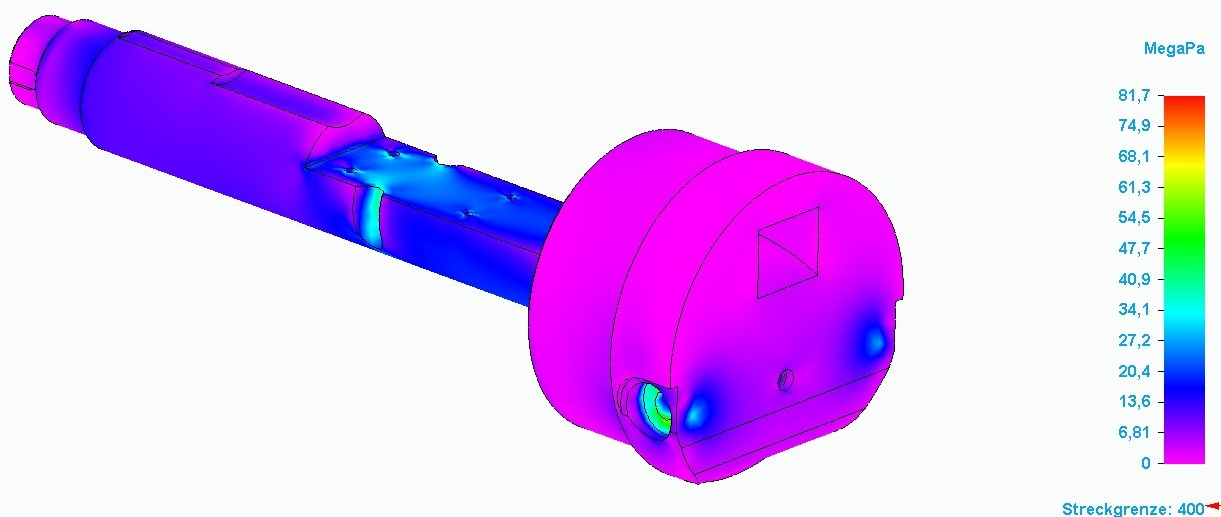
\includegraphics[width=0.9\textwidth]{FEM Welle.jpg}
	\caption{FEM-Ergebnisse der Welle}
	\label{abb_Well_FEM}
\end{figure}\\
Wie auch bei den Lagern ist die Dimensionierung der Welle nicht durch die mechanischen Lasten sondern geometrischen Randbedingungen bestimmt, sodass nirgends auch nur ansatzweise kritische Belastungen auftreten.
\\~\\
Mit einer Masse von $m=6,2$kg ist sie jedoch viel zu schwer. Wie in Abbildung \ref{abb_Well_FEM} klar zu sehen ist, besitzt sie jedoch viel Volumen, welches nicht benötigt wird und somit nur unnötigen Ballast darstellt. Somit zeigt Abbildung \ref{abb_abgespeckt}, wie eine massenreduzierte Version der Welle aussieht.
\begin{figure}[h] 
	\centering
	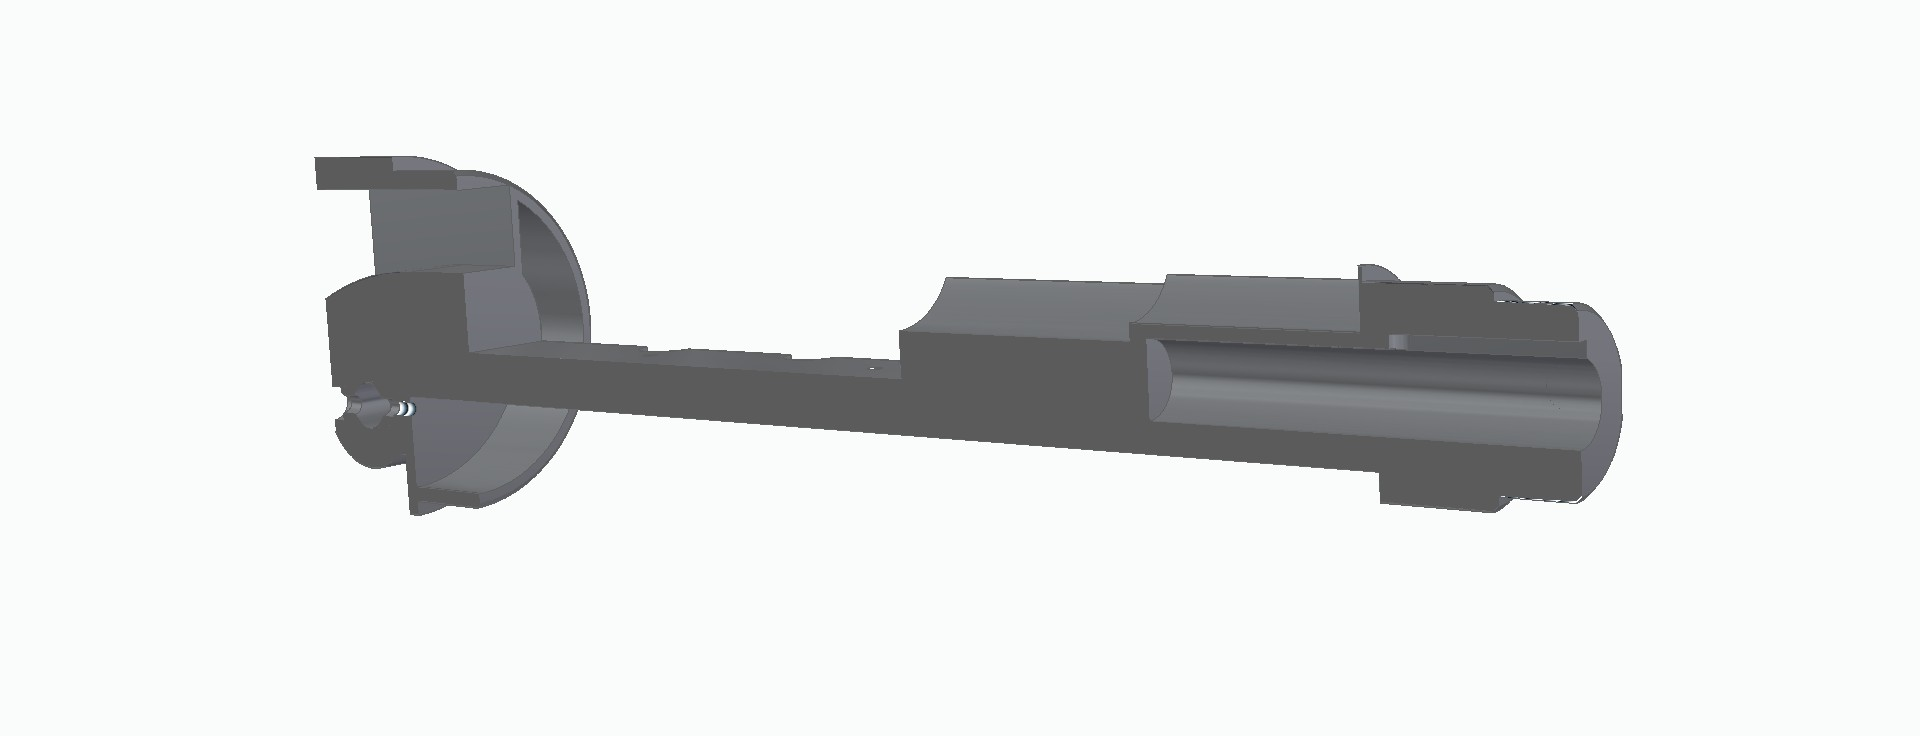
\includegraphics[width=0.75\textwidth]{Welle_abgespeckt_3D.jpg}
	\caption{Schnittanschicht der massenreduzierten Welle}
	\label{abb_abgespeckt}
\end{figure}\\ Besonders der vordere Teil mit dem großen Durchmesser trägt maßgeblich zur Masse bei. Diese Maße sind zwar nötig, um den Durchgang der Hubstange zu erlauben, aber der Innenraum kann ausgehöhlt werden. Auch der Einschnitt auf der Unterseite, der ein Anstoßen der Pfeilungsspitzen verhindert, kann ausgeweitet werden und ist nur durch die Durchgangsbohrung für die Verbindungswelle und der Notwendigkeit einer Wellenschulter für das Lager beschränkt. Auch auf der Oberseite des vorderen Wellenendes ist die Wellenschulter als Mindestradius notwendig. Zu den Bohrungslöchern für die Verbindungswelle muss die Oberfläche weiterhin nach außen laufen, um zum einen die Strömung nach außen abzuleiten und ein Auftreffen auf die planare Grid Fin Fläche zu verhindern und zum anderen die Verbindungswelle nicht über ihre Belastungsgrenze auf Biegung zu beanspruchen. Ergänzend kann auch noch in dem Abschnitt der Welle, in dem sich die Klappaktuatorik befindet, von der Unterseite Material angetragen werden. Am hinteren Ende beschränkt die Aufnahme für die Getriebewelle den Radius, aber die dafür vorgesehene Bohrung kann noch etwas verlängert werden, sodass der hintere Teil zur Hohlwelle wird. Somit hat sich die Masse der Welle drastisch auf einen Wert von nur noch $m= 2,2$ kg verringert. Auch mit diesen Veränderungen hält die Welle noch immer den Belastungen stand. Die FEM-Berechnung ergibt, dass noch immer nur maximal eine Spannung von $153$ MPa auftritt, und ihr Ergebnis ist in Abbildung \ref{abb_abgespecktFEM} zu erkennen.
\begin{figure}[h] 
\centering
\includegraphics[width=0.75\textwidth]{FEM Welle verstümmelt.jpg}
\caption{Schnittanschicht der massenreduzierten Welle}
\label{abb_abgespecktFEM}
\end{figure}
\subsection{Belastung des Gehäuses}
Abschließend wird noch das Aluminiumgehäuse betrachtet. Es hat nicht nur die Aufgabe, den Rest der Rakete von den beweglichen Teilen zu trennen, um zum Beispiel ein Verfangen von Kabeln zu verhindern, sondern auch die Funktion, die Lager und den Motor mit Getriebe in Position zu halten. Somit überträgt das Gehäuse auch die Kräfte und Momente, die in dem System wirken, auf den Raketenkörper. Für eine einfache Montage und Fertigung besteht das Gehäuse aus einer Unter- und Oberseite, die mit Schrauben aneinander und an der Außenhülle befestigt werden. Im vorderen Bereich benötigt die Oberseite der Welle auf Grund der Klappaktuatorik deutlich mehr Platz als auf der Unterseite. Deshalb bildet die Oberseite des Gehäuses einen Halbkreis, während die Unterseite eine halbe Ellipse darstellt, deren große Halbachse dem Radius der Oberseite entspricht, um bündig mit ihr abzuschließen. Hinter dem Kegelrollenlager sind beide Seiten symmetrisch aufbaut mit Ausnahme der Trennwände, die zur Unterseite gehören und an denen das Getriebe und der Motor montiert werden. Somit muss bei der Montage als letzter Schritt nur noch die Gehäuseoberseite auf die Unterseite platziert und dann befestigt werden.
Diese Befestigung findet mit der Raketenhülle mit sechs gleichmäßig über einen Flansch verteilte Schrauben statt. Mit zunächst sechs Schrauben, die über die gesamte Kontaktfläche verteilt sind, werden die beiden Gehäusehälften mittels Muttern miteinander verbunden.
\\~\\
Erneut wird hier eine FEM-Analyse benutzt, deren Ergebnis in Abbildung \ref{abb_FEM_Gehäuse1} zu sehen ist, um die Spannungen im Material zu bestimmen. Hierbei werden die Lagerkräfte auf die Flächen aufgebracht, auf denen die Lager aufliegen und gegendrücken. Das Moment um die Wellenachse wird über das Getriebe und den Motor auf das Gehäuse übertragen. Da das Getriebe eine Übersetzung von 200:1 besitzt und der Motor nur sehr kleine Momente liefert, wird vereinfacht angenommen, dass das gesamte Moment an Löchern für die Schrauben des Getriebes angreift.
\begin{figure}[h] 
	\centering
	\includegraphics[width=0.75\textwidth]{Gehäuse.jpg}
	\caption{Ergebnisse der FEM-Berechnung der Gehäusebaugruppe mit 6 Schrauben}
	\label{abb_FEM_Gehäuse1}
\end{figure}\\
Die Abbildung \ref{abb_FEM_Gehäuse1} zeigt, dass die Beanspruchungen im Material überall recht gering sind. Nur zwischen den Schrauben und Muttern kommt es zu hohen Belastungen mit Spannungen von bis zu $900$ MPa. Dies können Schrauben der Festigkeitsklasse 9.8 beziehungsweise 10.9 mit ihrer Zugfestigkeit bzw. Streckgrenze zwar erreichen, aber da sie als Normbauteile kostentechnisch kaum eine Rolle spielen, wird hier auf etwas mehr Sicherheit geachtet und die Anzahl der Schrauben von sechs auf zehn erhöht. Dies senkt die Spannung in den Schrauben deutlich ab, sodass ihre Belastung nicht mehr kritisch ist.\\
Da die Spannungen im Gehäuse fast nicht existent sind, kann die Wandstärke noch deutlich reduziert werden. Zuvor lag sie überall bei 4mm und wird nun auf 1mm reduziert. Nur der Flansch, an denen die beiden Gehäusehälften zusammengeschraubt werden, bleiben unverändert. Da die Kanten, an denen das Lager sitzt, sehr scharf sind, kommt es dort nun zu Spannungsspitzen, die über der Streckgrenze liegen. Deswegen werden die Auflagefläche des Kegellagers und die beiden angrenzenden Wände wieder auf eine Wandstärke von 4mm angehoben. Nun kommt es nur noch zu Spannungen von ca. 400MPa. Dies ist noch immer über der Streckgrenze von gängigen Aluminiumlegierungen, sodass versucht wird diese weiter zu senken. Also wird die Geometrie des vordersten Flansch direkt am Flansch für die Montage am Raketenkörper angepasst und Verrundungen an den kritischen Kanten hinzugefügt. Dadurch wird nun endgültig das angemessenes Gehäuse aus Abbildung \ref{abb_FEM_Gehäuse2} erreicht.
\begin{figure}[h] 
	\centering
	\includegraphics[width=0.75\textwidth]{Gehäuse 1mm 5 rundungen.jpg}
	\caption{Ergebnisse der FEM-Berechnung der endgültigen Gehäusegeometrie}
	\label{abb_FEM_Gehäuse2}
\end{figure}\\
\section{Betriebssimulation}\label{sec:betriebssim}
Da nun bewiesen wurde, dass die gesamte Konstruktion, die in Abbildung \ref{abb_gesamt_sys} gezeigt wird, den mechanischen Lasten des Betriebs stand hält, soll an dieser Stelle überprüft werden, ob die Antriebe über genug Leistung verfügen die gewünschten Manöver durchzuführen. Deswegen werden zur Überprüfung der Aktuatorik Betriebssimulationen in der Matlab-Anwendung Simulink durchgeführt.
\begin{figure}[h] 
	\centering
	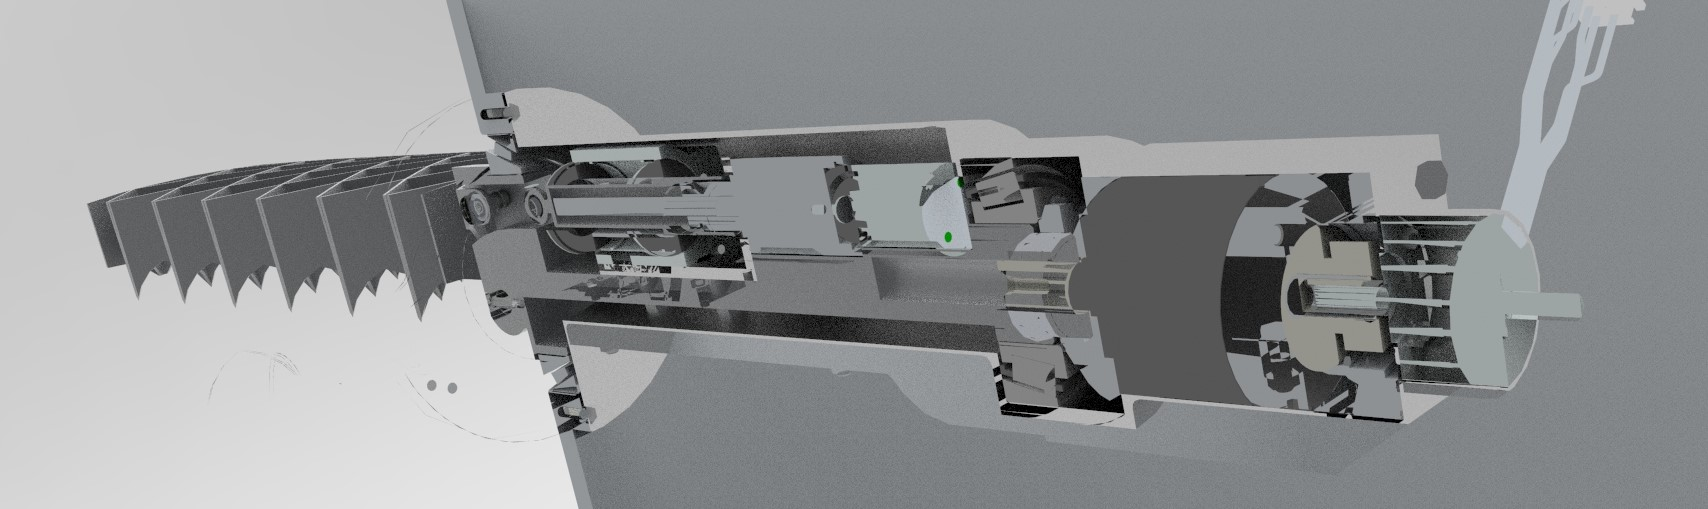
\includegraphics[width=0.8\textwidth]{System Render.jpg}
	\caption{Schnittansicht des Gesamtsystems}
	\label{abb_gesamt_sys}
\end{figure}
\subsection{Klappwinkel}
Zuerst wird der Prozess des Ausklappens simuliert. Dieses System besteht aus den drei in Abbildung \ref{abb_klappStrecke} gezeigten, miteinander verknüpften Teilen. 
\begin{figure}[h] 
	\centering
	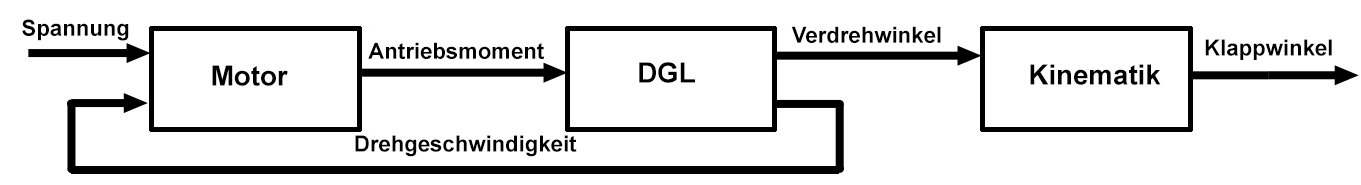
\includegraphics[width=\textwidth]{Schaubild Klapp.png}
	\caption{Schaubild der Strecke der Klappaktuatorik}
	\label{abb_klappStrecke}
\end{figure}\\
Das erste Subsystem stellt der Motor dar, dessen Kennlinie sich mit Gleichung \ref{eq_kennlinie} beschreiben lässt.
\begin{equation}\label{eq_kennlinie}
	M_{Motor} = (k_nU-n)\bigg(\frac{\Delta n}{\Delta M}\bigg)^{-1}
\end{equation}
$k_n$ ist dabei die Drehzahlkonstante des Motors und ist zusammen mit der Kennliniensteigung $\frac{\Delta n}{\Delta M}$ als konstante Kenngröße dem Datenblatt zu entnehmen. Die Spannung $U$ wird von außen angelegt und die Drehzahl $n$ ergibt sich aus der Lösung des Systems, sodass sich mit der Gleichung das Motormoment bestimmen lässt. Dieses Moment wird dann jedoch noch vom Getriebe auf Kosten der Drehzahl mit der Übersetzung $i = 200$ verstärkt, sodass sich das Antriebsmoment und umgekehrt die Motordrehzahl ergibt.
\begin{equation}
	M_\mathrm{Antrieb} = i \cdot M_\mathrm{Motor}
\end{equation}
\begin{equation}
	n_\mathrm{Motor} = i \cdot n_\mathrm{Antrieb}
\end{equation}
 Dieses Getriebe besteht zwar sowohl aus der Spindelstange, die die Rotations- in eine Linearbewegung umwandelt, als auch einem vorgeschalteten Planetengetriebe, jedoch wird im ersten Subsystem nur das Planetengetriebe berücksichtigt, während die Spindelstange vorerst vernachlässigt wird. Das Antriebsmoment wird dann an das zweite Subsystem weitergegeben, in dem die Differenzialgleichung
\begin{equation}
	\ddot{\varphi} = \frac{M_{Antrieb} - M_{R}}{I}
\end{equation}
gelöst wird. Die Beschleunigung des Trägheitsmoments $I$ um den Verdrehwinkel $\varphi$ hängt also von der Differenz des Antriebs- und Reibmoments ab. Letzteres ergibt sich aus dem Hebelarm $r$ und der Reibkraft des jeweiligen Kontaktpunktes, die wiederum vom Reibungsbeiwert $\mu$ und der Normalkraft $F_N$ abhängig ist und immer der Bewegung entgegenwirkt. Für das Getriebe ist zwar kein Reibungsbeiwert bekannt, aber eine Nenneffizienz $\eta$, sodass das sein Reibmoment als ein nur vom Antriebsmoment abhängiger Wert angenommen wird.
\begin{equation}\label{eq_reibmoment}
	M_R = M_{Antrieb}\cdot(1-\eta)+\frac{\dot{\varphi}}{|\dot{\varphi}|}\sum F_N \mu r
\end{equation}
Das Trägheitsmoment setzt sich aus Trägheitsmomenten der einzelnen Bestandteile der Aktuatorik zusammen, welche je nach Kinematik noch entsprechend umgerechnet werden müssen.

Aus dem Ergebnis dieser Differenzialgleichung, die Drehbeschleunigung $\ddot{\varphi}$, lässt sich dann zum einen die Drehgeschwindigkeit $\dot{\varphi}$ mittels einfacher und der Verdrehwinkel $\varphi$ mit zweifacher Integration bestimmen. Die Drehgeschwindigkeit wird zum einen für die Richtung des Reibmoments, wie es in Gleichung \ref{eq_reibmoment} zu sehen ist, benötigt und zum anderen für eine Umrechnung zur Drehzahl an den Motor zurückgegeben. Der Verdrehwinkel hingegen wird an das dritte und letzte Subsystem, welches sich mit der Geometrie der Kinematik beschäftigt, weitergeleitet.
\begin{figure}[h] 
	\centering
	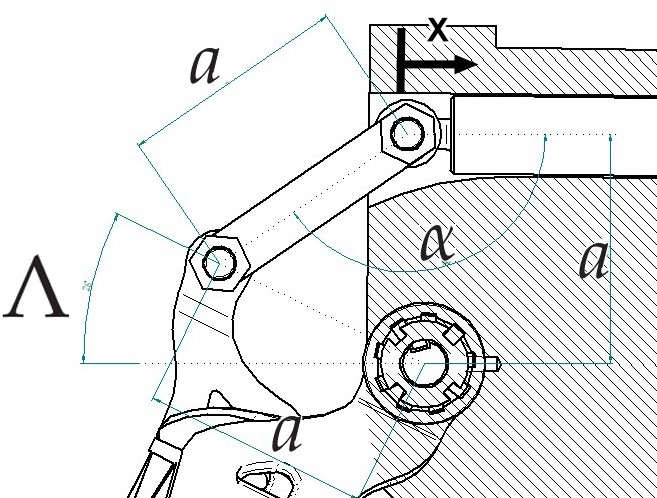
\includegraphics[width=0.5\textwidth]{KinKlapp.jpg}
	\caption{Kinematischer Zusammenhang von Hubweg und Klappwinkel}
	\label{abb_kinklapp}
\end{figure}\\

Hier wird die Verdrehung über die Steigung der Spindelstange erst in eine Linearbewegung der Hubstange und dann wieder in die Rotation des Grid Fins um den Klappwinkel $\Lambda$ umgewandelt. Abbildung \ref{abb_kinklapp} zeigt, wie aus den geometrischen Zusammenhängen sich zuerst der Winkel
\begin{equation}
	\alpha=\arcsin\bigg(1-\frac{x}{a}-\cos(\Lambda)\bigg)
\end{equation}
in Abhängigkeit vom Hubweg $x$ ergibt, der dann genutzt werden kann, um den Klappwinkel
\begin{equation}
	\Lambda = \arcsin\bigg(1-\sin(\alpha)\bigg)
\end{equation}
zu bestimmen.
\begin{figure}[h] 
	\centering
	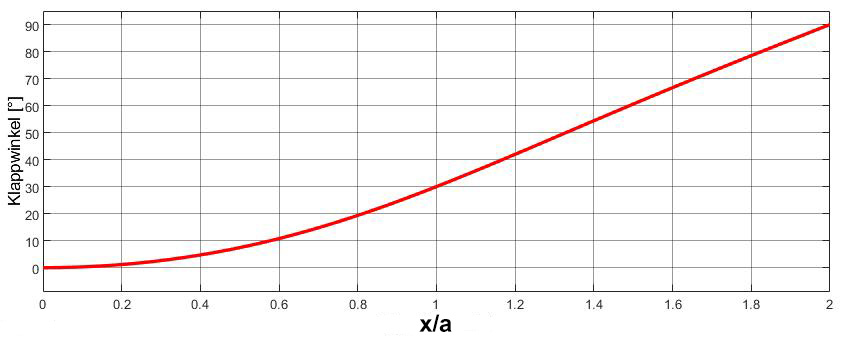
\includegraphics[width=0.9\textwidth]{KinKlappGraph.jpg}
	\caption{Klappwinkel $\Lambda$ in Abhängigkeit vom normalisierten Hubweg $x/a$}
	\label{abb_KinKlappGraph}
\end{figure}\\	
Sobald der Klappwinkel von $\Lambda = 90^\circ$ erreicht wird, beziehungsweise wenn die Hubstange sich um eine Länge von $x = 2a = 75$ mm bewegt hat, stößt sie gegen das Getriebe und eine weitere Bewegung in diese Richtung ist nicht mehr möglich. Wenn dieser Fall eintritt, wird die Spannung am Motor auf null gesetzt und das Manöver gilt als beendet.
\\
Abbildung \ref{abb_KinKlappGraph} zeigt, dass der Verlauf des Klappwinkel in Abhängigkeit vom normalisieren Hubweg $x/a$ erst mit nur sehr geringer Steigung beginnt, doch dann ab $x/a \approx 0.8$ einen fast linearen Verlauf annimmt. Sowohl das Trägheitsmoment, mit dem der Grid Fin im Subsystem der Differenzialgleichung wirkt, als auch die Kraft in den Lagern, die zur Reibung führt, hängen vom aktuellen Klappwinkel ab und sind somit nicht konstant. Da jedoch schon der Klappwinkel rekursiv errechnet werden muss, ist es nicht möglich in Simulink einen weiteren geschlossenen Kreis mit diesem Wert zu bilden. Stattdessen werden Vereinfachungen angenommen. Es wird die lineare Steigung im hinteren Bereich des Verlaufs aus Abbildung \ref{abb_KinKlappGraph} als konstanter Wert für die Rechnung verwendet. Dies ist eine konservative Annahme, da die geringere Steigung im vorderen Bereich nur schwächere Reibungskräfte und Trägheitsmomente bewirken würde. Die Kraft in den beiden Kugellagern ergibt sich aus dem Trägheitsmoment des Grid Fins mit der Annahme eines Ausklappens innerhalb von zwei Sekunden. Es wird angenommen, dass in beide Lager jeweils das gesamte Moment mit dem Hebelarm $a$ aufnehmen. Da außer der Trägheit in der Schwerelosigkeit keine Kräfte wirken, wird davon ausgegangen, dass die Reibung im Linearlager zu vernachlässigen ist. Wegen des geringen Reibungsbeiwertes $\mu = 0.0015$ \cite{lagerreibung} von Kugellagern ist die Reibung im Getriebe um drei Größenordnungen größer und somit von deutlich entscheidenderer Bedeutung.

Wird nun die Simulation mit der Nennspannung von $U = 12$ V durchgeführt, zeigt Abbildung, dass der Grid Fin innerhalb von weniger als 2,9 Sekunden ausklappt. Dies liegt weit unter der Zeitspanne zwischen Separation und ReEntry-Burn, die maximal zur Verfügung steht. Der Motor ist für die Anwendung also eigentlich zu leistungsstark. Da jedoch trotz der reduzierten Masse des Grid Fins kein anderes dimensioniertes Spindelgetriebe in Frage kommt, ist dieser Motor noch immer die günstigste Option.
Als Effizienz $\mu$ des Getriebes ist jedoch nur ein Maximalwert gegeben, der hier auch verwendet wurde. Selbst wenn dieser von $\mu = 0,75$ auf einen sehr niedrigen Wert von $0,25$ herabgesetzt wird und nur noch eine Spannung von $U = 4$ V am Motor anliegt, klappt der Grid Fin noch immer innerhalb von ungefähr 8,5 Sekunden aus.

Dies zeigt, dass nicht wie bisher eine Spindelstange mit einem reibungsarmen Kugelumlaufgewinde verwendet werden muss. Stattdessen kann auf ein Trapezgewinde zurückgegriffen werden, welches mit $\eta  = 0,38$ eine deutlich geringere Effizienz hat, aber trotzdem noch immer ausreicht. Bei $U = 4$ V braucht der Grid Fin noch immer nur 7,4 Sekunden zum Ausklappen. Abbildung \ref{abb_klappKG} zeigt, dass der die Zeitdifferenz trotz den großen Unterschieds im Wirkungsgrad gering bleibt. Der Preis für das Spindelgetriebe sinkt aber signifikant von 768€ auf 513€.
\begin{figure}[h] 
	\centering
	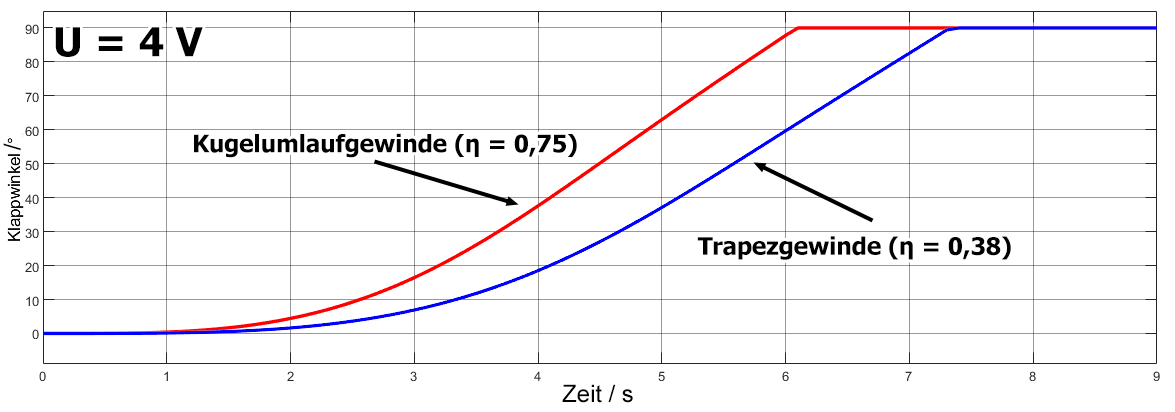
\includegraphics[width=0.8\textwidth]{Klapp3 mixed.png}
	\caption{Klappbewegung des Kugelumlaufgewinde und Trapenzgewinde bei 4 V im Vergleich}
	\label{abb_klappKG}
\end{figure}\\
Der in Abbildung \ref{abb_klappKG} dargestellt Verlauf des Klappwinkels zeigt einen Knick bei $Lambda = 90^\circ$. Dies kommt dadurch zustande, dass der Motor konstant mit der gleichen Spannung betrieben wird, bis die Hubstange ungebremst gegen das Spindelgetriebe stößt.
\begin{figure}[h] 
	\centering
	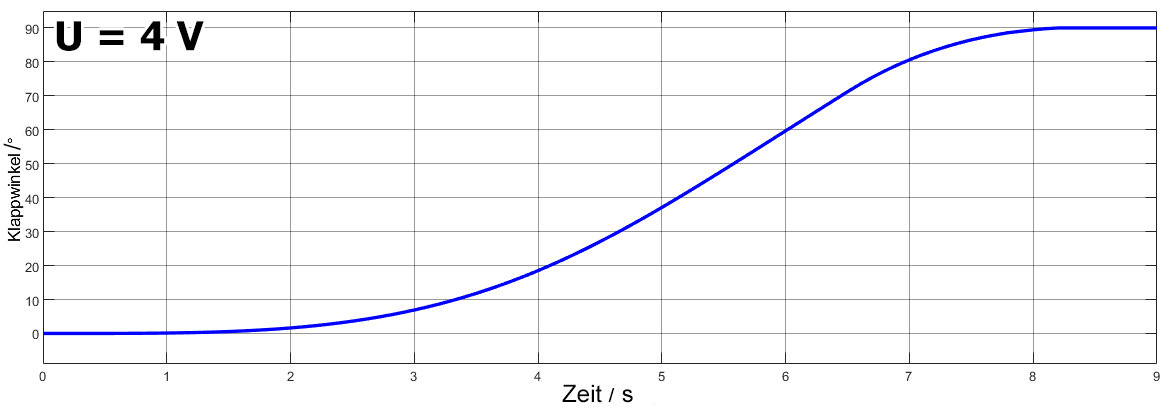
\includegraphics[width=0.8\textwidth]{klapp_geregelt.png}
	\caption{Klappbewegung mit Trapezgewinde und PI-Regler}
	\label{abb_klappPI}
\end{figure}
Dies lässt sich verhindern, indem, wie es beim Steuerwinkel gemacht werden soll (vgl. Abbildung \ref{abb_steuerStrecke}, ein PI-Regler zusätzlich eingebaut wird. Abbildung \ref{abb_klappPI} zeigt, dass sich mit Regelung die Kurve abrundet. Die für das Manöver benötigte Zeit steigt dadurch um ungefähr eine Sekunde auf $8,1$ s. 
\subsection{Steuerwinkel}
Das Schaubild in Abbildung \ref{abb_steuerStrecke} zeigt den Aufbau der Betriebssimulation für den Steuerwinkel.
\begin{figure}[h] 
	\centering
	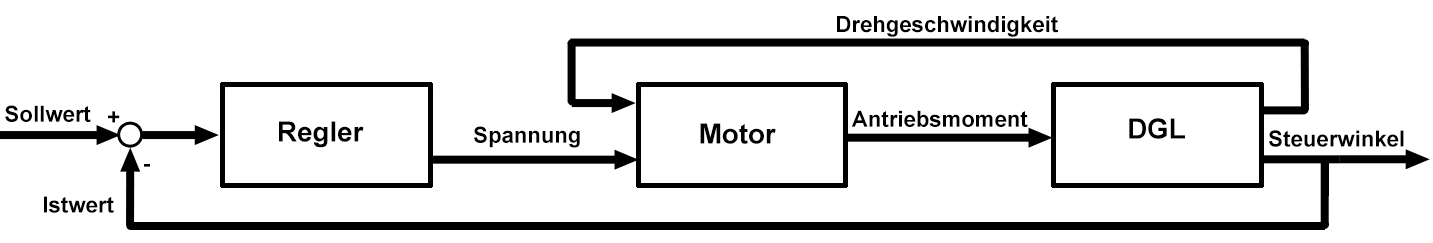
\includegraphics[width=\textwidth]{Schaubild Steuer.png}
	\caption{Schaubild der Regelstrecke der Steueraktuatorik}
	\label{abb_steuerStrecke}
\end{figure} 
Das Subsystem des Motors bleibt vom Aufbau her unverändert und kann ohne Weiteres von der Klappwinkelsimulation übernommen werden. Auch die Differenzialgleichung hat grob die gleiche Struktur.
\begin{equation}
	I\ddot{\delta} = M_{Antrieb} - M_{R} - M_{m}
\end{equation}
Zu den Momenten, die auch schon beim Klappwinkel vorkamen, kommt nun auch das aerodynamische Gelenkmoment $M_m$ dazu. Dieses wird als linear vom Steuerwinkel $\delta$ abhängig angenommen, was sich bei den Analysen von Miller und Washington \cite{synopsis} (vgl. Abbildung \ref{abb_krumm}) erkennen lässt. Somit ergibt sich
\begin{equation}
	M_{m} = \frac{M_{m, \mathrm{max}}}{\delta_\mathrm{max}} \cdot \delta =\frac{89,1\mathrm{Nm}}{20^\circ} \cdot \delta = 4,455\frac{\mathrm{Nm}}{^\circ}\cdot \delta.
\end{equation}
Der Anteil des Reibungsmoments aus der Lagerreibung lässt sich für den Steuerwinkel auch einfacher ermitteln, da sie sich aus den am Grid Fin angreifenden Kräften bestimmen lassen. Hierfür können die in Abschnitt \ref{sec:lagerWelle} zur Lagerung der Welle verwendeten Formeln \ref{eq_lagerWelle1} und \ref{eq_lagerWelle1} verwendet werden. Auch wenn der Reibungsbeiwert von Kegelrollenlagern leicht höher ist als der von Rillenkugellagern \cite{lagerreibung}, ist die Bedeutung der Lagerreibung gegenüber den Verlusten im Getriebe noch immer vernachlässigbar gering.

Da die Variable der Differenzialgleichung schon der gewünschte Steuerwinkel $\delta$ ist, ist kein drittes Subsystem für eine Transformation der Kinematik nötig. Die Bewegung, die durchgeführt werden soll, ist jedoch komplexer als beim Klappwinkel, sodass die anliegende Spannung nicht konstant gehalten werden kann. Deswegen wird ein PI-Regler eingebaut, der in Abhängigkeit vom Steuerwinkel die Spannung regelt.
Weil eine komplette Schwingung innerhalb von $T = 0,73$s stattfinden soll, wird der Sollwert für den Steuerwinkel bis $t = 1/4T$ auf $\delta = 20^\circ$ gesetzt. Danach springt der Wert auf $\delta = -20^\circ$. Ab $t = 3/4T$ soll Steuerwinkel wieder auf $\delta = 0^\circ$ zurückgehen. Von dort war er auch mit einer Drehrate von $\dot{\delta} = 0$ rad/s gestartet.
Der Regeler ist jedoch keineswegs für die Anwendung optimiert und dient nur der Demonstration der Fähigkeit des Motors genug Leistung aufzubringen, um dieses Manöver durchzuführen.

Der gewählte Motor hat eine Nennspannung von $U = 12$V, die zunächst als Maximum festgelegt wird. Abbildung \ref{abb_steuerNenn} zeigt aber, dass der Motor unter diesen Bedingungen gerade mal einen Steuerwinkel von $\delta = \pm 12^\circ$ einzustellen schafft.
\begin{figure}[h] 
	\centering
	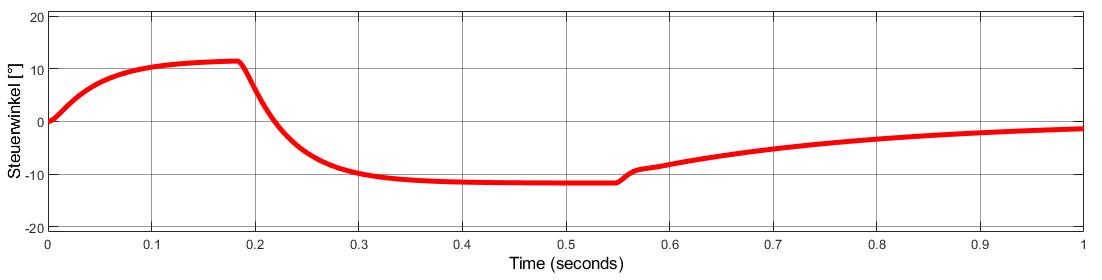
\includegraphics[width=\textwidth]{Steuer12V.png}
	\caption{Steuerwinkel in Abhängigkeit von der Zeit bei Nennspannung}
	\label{abb_steuerNenn}
\end{figure}\\
 Jedoch ist die Nennspannung nur für den Dauerbetrieb als Grenzwert anzusehen. Da aber der Wiedereintritt in die Atmosphäre, in der dieses Manöver durchgeführt wird, nur circa 40 Sekunden dauert, wobei nur in einem Intervall von ungefähr 20 Sekunden die hohen aerodynamischen Kräfte auftreten, ist die meiste Zeit gar nicht eine so hohe Leistung notwendig. Mit einer thermischen Zeitkonstante der Wicklung von $11,8$s ist ein Überschreiten der Nennspannung um ihr Vielfaches nicht sofort schädlich. Deutlich höher muss die Spannung aber auch gar nicht gesteigert werden. Wie Abbildung \ref{abb_Steuer18V} zeigt, reicht schon eine Spannung vom 1,5-fachen der Nennspannung aus, um die Bewegung wie gewünscht durchzuführen. Die Steueraktuatorik ist aber deutlich sensibler gegenüber unerwarteten Störungen als der Klappaktuator. Bei geringerer Maximalspannung und einer Senkung der Getriebeeffizienz um mehr als 5\% kann er unter den Maximalbedingungen nicht mehr die gewünschte Bewegung ausführen.
\begin{figure}[h] 
\centering
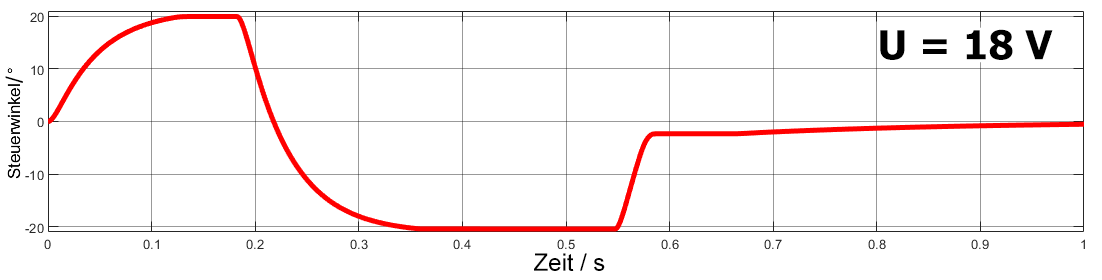
\includegraphics[width=\textwidth]{Steuer18V.png}
\caption{Steuerwinkel in Abhängigkeit von der Zeit bei 1,5-facher Nennspannung}
\label{abb_Steuer18V}
\end{figure}\\
\section{Systembewertung und Fazit}
Es wurde eine Grid Fin Aktuatorik für wiederverwendbare Raketen, die unter extremen Wiedereintrittsbedingungen einsatzfähig bleibt, entworfen. Nicht nur der Grid Fin an sich hält den mechanischen Belastungen stand, die durch die aerodynamischen Kräfte bewirkt werden, sondern auch die Bauteile, an denen er befestigt ist, können diese Spannungen ertragen und in den Raketenkörper weiterleiten. Dabei wird nicht von einem planmäßigen Wiedereintritt mit ReEntry-Burn ausgegangen, sondern das Worst-Case-Szenario angenommen, bei dem die Rakete ungebremst auf die Atmosphäre trifft. Die größten Bedenken gelten hierbei der thermischen Belastung, die weiterhin eine große Unbekannte ist. Sie konnte bisher noch nicht berücksichtigt werden und könnte somit zum Totalversagen des Systems durch Schmelzen des Gittermaterials führen.
\\~\\
Das System muss aber nicht nur den Belastungen standhalten, sondern auch eine Beweglichkeit um zwei Achsen in bestimmten Grenzen erlauben. Der erste Aktuator steuert den Grid Fin beim Wiedereintritt und schafft es selbst bei den harschen Bedingungen ohne ReEntry-Burn eine Bewegung von $\pm 20^\circ$  innerhalb von weniger als 0,73 Sekunden auszuführen. Obwohl er nur recht knapp ausgelegt ist und schon bei leicht erschwerten Bedingungen nicht mehr in der Lage ist, die Bewegung auszuführen, wird er dennoch den Anforderungen gerecht. Der Aktuator zum Ausklappen der Grid Fins nach der Stufentrennung und vor dem Wiedereintritt ist deutlich robuster ausgelegt. Er schafft es innerhalb kürzester Zeit seine Funktion zu erfüllen und danach die Position zu halten. Dieser Aktuator kann auch noch bei deutlich erschwerten Bedingungen seine Aufgabe erfüllen.
\\~\\
Auch wenn einige Komponenten natürlich maßgefertigt werden müssen, insbesondere der Grid Fin, die Welle und das Gehäuse, wurden so weit wie möglich COTS verwendet. So sind die Motoren, Getriebe und Lager alle von Anbietern online bestellbar, ganz abgesehen von den Normbauteilen, die wie Schrauben und Muttern teilweise sogar aus dem lokalen Baumarkt in geringen Stückzahlen erhältlich sind. Die restlichen Bauteile sind aus einfachen Halbzeugen mit nur wenigen Arbeitsschritten fertigbar. Dadurch werden Kosten auf ein Minimum begrenzt. Für COTS ergeben sich somit pro Grid Fin Gesamtkosten von etwas über 1.600€. Die Gesamtmasse pro Aktuatorik inklusive Grid Fin beläuft sich auf ungefähr $8,7$kg. Der Grid übersteigt diese Kosten mit einem Preis von 13.000€ im 3D-Druck bei weitem.
\\~\\
Zusammenfassend lässt sich sagen, dass die Aktuatorik alle geforderten Funktionen erfüllt. Sie hält allen zu berücksichtigenden Belastungen stand und ermöglicht die Bewegung der geforderten Freiheitsgrade. Somit wurden alle im Rahmen dieser Arbeit gestellten Anforderungen erfüllt.
